\documentclass[twocolumn,superscriptaddress,showpacs,prl,nofootinbib,floatfix]{revtex4}
\usepackage{graphicx,epsfig,psfrag}
\usepackage{amsmath}
 
 \usepackage{wasysym} 
 \usepackage{mathrsfs} 
 \usepackage{graphicx} 
 \usepackage{amsfonts} 
 \usepackage{amsbsy} 
 \usepackage{amscd} 
 \usepackage{amssymb}
 %\usepackage{bbm}  
 %\usepackage{accents} 
 \usepackage{pstricks} 
 \usepackage{multirow} 
 
  
%%%%%%%%%%%%%%%%%%%%%%%
%% Elsevier bibliography styles
%%%%%%%%%%%%%%%%%%%%%%%
%% To change the style, put a % in front of the second line of the current style and
%% remove the % from the second line of the style you would like to use.
%%%%%%%%%%%%%%%%%%%%%%%

%% Numbered
%\bibliographystyle{model1-num-names}

%% Numbered without titles
%\bibliographystyle{model1a-num-names}

%% Harvard
%\bibliographystyle{model2-names.bst}\biboptions{authoryear}

%% Vancouver numbered
%\usepackage{numcompress}\bibliographystyle{model3-num-names}

%% Vancouver name/year
%\usepackage{numcompress}\bibliographystyle{model4-names}\biboptions{authoryear}

%% APA style
%\bibliographystyle{model5-names}\biboptions{authoryear}

%% AMA style
%\usepackage{numcompress}\bibliographystyle{model6-num-names}

%% `Elsevier LaTeX' style
\bibliographystyle{elsarticle-num}
%%%%%%%%%%%%%%%%%%%%%%%

\def\beq{\begin{equation}}
\def\eeq{\end{equation}}
%
\def\beqa{\begin{eqnarray}}
\def\eeqa{\end{eqnarray}}
%
%\def\bar{\begin{array}}
%\def\ear{\end{array}}
%
\def\ben{\begin{enumerate}}
\def\een{\end{enumerate}}
%
\def\bit{\begin{itemize}}
\def\eit{\end{itemize}}

\setlength{\mathindent}{0pt}


%%%%%%%%%%%%%%%%%%%%%%%


\begin{document}

%\begin{frontmatter}

%\title{Pure Majorana and Dirac-type  \\ 
%heavy neutrino states at the LHC}

\title{Dirac-ness of massive neutrinos composed of Majorana states}


%\tnotetext[mytitlenote]{Fully documented templates are available in the elsarticle package on \href{http://www.ctan.org/tex-archive/%macros/latex/contrib/elsarticle}{CTAN}.}

%\tnotetext[t1]{This article is registered under preprint number: 1504.05568 [hep-ph]}

%% Group authors per affiliation:
%% or include affiliations in footnotes:
\author{Janusz Gluza}
%\ead{janusz.gluza@us.edu.pl}
\affiliation{Institute of Physics, University of Silesia, Uniwersytecka 4, 40-007 Katowice, Poland}
\author{Tomasz Jeli\'nski}
\affiliation{Institute of Physics, University of Silesia, Uniwersytecka 4, 40-007 Katowice, Poland}
%\cortext[ca1]{Corresponding author}
%\ead{tomasz.jelinski@us.edu.pl}
\author{Magdalena Kordiaczy\'nska}
\affiliation{Institute of Physics, University of Silesia, Uniwersytecka 4, 40-007 Katowice, Poland}
%\ead{mkordiaczynska@us.edu.pl}
\author{Robert Szafron}
%\ead{szafron@ualberta.ca}
\affiliation{Department of Physics, University of Alberta, Edmonton, Alberta, Canada T6G 2G7}
%\fntext[myfootnote]{Since 1880.}


\begin{abstract}
Majorana neutrinos lead naturally to Lepton Flavour Violation (LFV). 
Representative LFV processes both at low energy physics and high energy hadron and lepton collisions are discussed. It is shown when a superposition of Majorana states mimic Dirac type of neutrinos, leading to recovery of the Lepton Flavour Conservation (LFC). A strength of LFV is a measurable quantity, which in turn gives correlations among Majorana neutrino parameters at the level of mixing or mass matrices, thus revealing possible details of neutrino mass generation mechanism. As far as TeV massive neutrinos are concerned, which are searched presently at the LHC, an example of possible neutrino parametrization is discussed which is in agreement with low energy stringent LFV  processes. This parametrization 
goes beyound simplified ATLAS and CMS analysis done so far and is proposed as a next step in direction of more complete  future 
LHC searching analysis.  
 
%Fine details are investigated which might influence determination of the heavy neutrinos nature at the  prominent $pp \to ll jj$ dilepton process.  
%Effects of the flavour mixings, decay widths, CP phases, Majorana heavy neutrino mass non-degeneracy and  lepton flavour violating restrictions are taken into account. In order to  discuss details quantitatively, the  CMS $\sqrt{s}=8$ TeV anomaly dilepton signals are considered. These data are in favour of a phase-Dirac type of neutrino, compounds of two Majorana degenerate heavy mass states with not maximal mixing and non-trivial CP phase. However, for  heavy neutrinos decay widths at the GeV level, the second scenario can be realized by apparently non-degenerate heavy Majorana mass states. Independently of possibles scenarios, the analysis suggests that more refined CMS and ATLAS analysis are desirable in the future, departing from trivial degenerate neutrino mass scenarios and trivial neutrino mixing matrices. 
%Such a non-degeneracy can be probed in future lepton colliders. 
%Based on our parametrization, a prediction for the LHC-2 $\sqrt{s}=14$ TeV dilepton signals is given. In addition, Higgs bosons contributions to the dilepton signal are estimated, taking into account theoretical and experimental restrictions on the mass spectrum of the minimal left-right symmetric model including bidoublet and triplet fields. 
%Due to these constraints,  scalars effects are tiny. 
\end{abstract}

%\begin{keyword}
%Left-Right symmetry\sep heavy neutrinos\sep right-handed currents \sep CP phases
%\end{keyword}

%\end{frontmatter}

%\linenumbers


\maketitle 
\allowdisplaybreaks


\section{Introduction}

%Since the beginning 
Neutrino physics is full of surprises with many  experimental measurements which not always survived but which in a meantime, quite often, led to bold, interesting or even weird theoretical interpretations. 

Presently, due to neutrino oscillation phenomenon, it is already established that three known neutrinos are massive, though their masses are very tiny, at the electronovolt level. Commonly we call them all the light (active) neutrinos. It was a long story which led to this result, started around a half century ago with a Homestake experiment and the so-called solar neutrino problem, leading finally to the discovery of the first type of neutrino oscillations \cite{Bahcall:1976zz}. About three decades ago, evidence for a 17-keV neutrino mass state (also called a Simpson's neutrino) coupled to the electron neutrino in nuclear decay spectra measurements made another huge controversy. The unclear situation lasted more or less during the period 1985-1993. Finally, this neutrino anomaly has been resolved and the Simpson's neutrino disappeared (in some experiments even 8 $\sigma$ C.L. have been announced). For a review on this issue, see e.g. \cite{Wietfeldt:1995ja,Franklin:1995pk}.  
On the way there were yet another controversies connected with neutrinoless doubly beta decay signals (see comments in \cite{Akhmedov:2014kxa}), or more recently, in the OPERA experiment.
Especially the last result excited not only physics society but also media through the world. Finally we are again in a trivial world where neutrinos are not faster than light \cite{Antonello:2012hg}. 

Certainly, we can expect more such situations in the future, as neutrino experiments explore very tiny and by definition {\it weak} effects and belong to one of the most challenging experiments in physics, ever. 
%No wonder that due to their hardly detectable and mysterious nature, neutrinos  they  making also excitement in public.
%\footnote{No wonder that due to their hardly detectable and mysterious nature, neutrinos are a thankful topic also in literature and movies. Maybe the best example comes from the "2012" catastrophic movie by  Roland Emmerich where "The neutrinos suddenly act like ... microwaves". This is of course artistic imagination, even more "drastic" cases of neutrinos misinterpretations can be easily found elsewhere.}

A year ago  another puzzle has been reported by the CMS Collaboration  which deals with products of proton-proton collisions at Large Hadron Collider (LHC) \cite{Khachatryan:2014dka}.  This time a concern is about  production and subsequent decay of hypothetical  heavy neutrinos $N$,  associated with right-handed currents and a new charged gauge boson $W_2$. CMS report triggered a lot of theoretical activity
and  was a fruitful seed for new ideas in quest of New Physics at the LHC  \cite{Deppisch:2014qpa,Heikinheimo:2014tba, Deppisch:2014zta,Aguilar-Saavedra:2014ola, Ng:2015hba,Dobrescu:2015qna,Brehmer:2015cia,Dev:2015pga,Coloma:2015una,Gluza:2015goa,
Das:2014jxa} \footnote{Interesting before CMS era works are \cite{Han:2012vk, Atre:2009rg}...gdzie indziej For  interpretations of the CMS signals not connected with neutrino physics, see \cite{Berger:2015qra,Krauss:2015nba,Dhuria:2015swa}. Interestingly, there are also other channels where TeV resonances are discussed, e.g. diboson channels cite...}. 
CMS reported 13 electron-positron-jet-jet ($e^+e^-jj$) events which are beyound the Standard Model analysis. Second, one additional event which breaks the lepton number was identified ($e^-e^-jj$). Finally, no excess connected with muon pair production ($\mu \mu jj$) has been found. 

Why these, should be said honestly, still statistically dim events are so spectacular and excited many theoreticians so much? The shortest answer is: 13 LFC $e^+e^-jj$ events over a single LFV  $e^-e^-jj$ event indicates that heavy neutrinos are of pseudo-Dirac nature. Meaning: they brake lepton number only slightly, and this calls for proper theoretical interpretations\footnote{If $e^-e^-jj$ event is misidentified, then excesses are only due to LFC events, which can be explained by Dirac neutrinos, as discussed in dobrescu.}.  
%Even if signals melt out with better statistics, digging the issue of LFV  

A hunt for LFV low and high energy processes in particle physics is a decades long story. Fact is that even single LFV event detection  would be a signal for New Physics. Present bounds for low energy LFV signals, such as 
% For that we will consider not only collisions at hadron or lepton colliders but also low energy processes as LFV 
$\mu \to e \gamma$  are already impressive, and they should increase very much in the future, at the so-called intensity frontier experiments where
New Physics can be probed up to unimaginable 10 000 TeV scale cite-Robert, which is four orders of magnitudes higher  than capabilities of present or doubtless future high energy colliders energies cite 
 
If heavy neutrinos have to do anything with the CMS anomaly, their masses are presumable about trillion times larger than masses of known light neutrinos (i.e. $M_{N}\sim $ TeV). 
%Such TeV  mass scale particles can be probed at the LHC and substantial signals, responsible for the excess effects, can be obtained. 
There is a good theoretical reason for such heavy states. Popular see-saw mechanism has been constructed  to explain smallness of the known light neutrino mass states cite(). Here neutrinos are naturally of Majorana nature, they are self-conjugate and can lead to the Lepton Flavour Violation processes cite. Alternatively, there is also another  interesting mechanism,  inverse seesaw, in which also pseudo-Dirac
neutrinos can appear cite. Here LFV can vary more naturally and can be large or small.

  Our main focus is to show how starting with Majorana neutrinos and an
  effective right-handed charged current, a strength of LFV can change in physical processes. 
%  nie wiem czy brnac w to, chyba nie: We may argue on many levels which neutrinos are more natural: Dirac or Majorana. We prefer Majorana fields as a more economic choice in QFT, cite jakies textbook,  for instance,  and this is our starting point. 
  First reason for LFV can be a mixing of flavour Majorana states, however, other factors can affect signals either: decay widths, CP phases, and Majorana heavy neutrino mass splittings. Settling down these issues, our final goal is to convience a reader that such fine details are important for experimental analysis, e.g. just mentioned CMS data cite or 
  ATLAS analysis to which we will come. 
  
  In what follows,  we will consider not only some hadron or lepton colliders collisions, which may lead to LFV, but also prominent low energy processes of this kind. 
  
\section{Right-handed currents and LFV at the LHC and at the intensity frontier}

%potrzebne??? We will not focus on mechanisms which might generate light and heavy neutrino states, they can go equally well beyond direct or inverse seesaw mechanisms.
%Let us instead assume that  
Our discussion will be based on the following lagrangian

\begin{eqnarray}
\mathcal{L}&\supset& \frac{{g}}{\sqrt{2}}\sum\limits_{a=1}^3\overline{\nu}_a\gamma^{\mu}P_L(U_{PMNS})_{aj}l_jW_{1\mu}^{+}
%\cos\xi
+\mathrm{h.c.}  \;\;\;\;\;\;\;\;\;\;\;\;\label{lagr1} \\
&+&\frac{\tilde{g}}{\sqrt{2}}\sum\limits_{a=1}^3\overline{N}_a\gamma^{\mu}P_R(K_{R})_{aj}l_jW_{2\mu}^{+} +\mathrm{h.c.} \;\;\;\;\label{lagr2}
%\\
%&&-\frac{g_L}{\sqrt{2}}\overline{N}_a\gamma^{\mu}P_R(K_{R})_{aj}l_jW_{1\mu}^{+}\sin\xi+\mathrm{h.c}.
%
%\label{lagr3}\\
%
%&&+\frac{g_L}{\sqrt{2}}\overline{l}_iP_-\gamma^{\mu}
%%\underbrace{
%(K_{R})_{bi}^*
%%}_{(K_{R}^\dag)_{ib}}
%N_bW_{2\mu}^{-}\,.\label{lagr2}
\end{eqnarray}

Eq.\ref{lagr1} describes the SM physics of charged currents. It includes the neutrino mixing matrix 
$U_{PMNS}$, responsible for neutrino oscillations phenomena. Eq.\ref{lagr2} is responsible for non-standard effects connected with new heavy neutrino massive states $N_a$ and right-handed currents mediated by additional heavy charged gauge boson $W_2$. 


In further discussion we assume that $N_a$ are heavy flavour neutrino states which are composed of Majorana massive states $N_i$, $N_a = \sum\limits_{i=1}^3 {(K_R)}_{ai} N_i$. 
$K_R$ is with a good approximation a unitary mixing matrix which diagonalizes heavy neutrino sector leading to the $N_i$ massive states. 
$\tilde{g}$ is a gauge coupling equal to the SM gauge coupling $g$, or smaller, if we wish  strict gauge coupling unification cite...

%Of course, we can assume from the beginning that underlying theory includes Dirac neutrinos, which at some situations be zaleta, see e.g. dobrescu.
 
%A key feature of the CMS analysis is that the  excess of the opposite-sign  (OS) leptons of the first generation (electrons and positrons) $e^+ e^- jj$ is observed, not accompanied by an excess in
%the same-sign (SS) $e^- e^- jj$ and $e^+ e^+ jj$ final states. In addition, no excess in leptons signals of the second generation ($\mu\mu$ channel) has been reported \cite{Khachatryan:2014dka,Khachatryan:2015gha}. 

The CMS excess in dilepton data mentioned in the Introduction can be explained by the process 
schematicaly sketched in Fig.~\ref{lljj}
\begin{figure}[h!]
\begin{center}
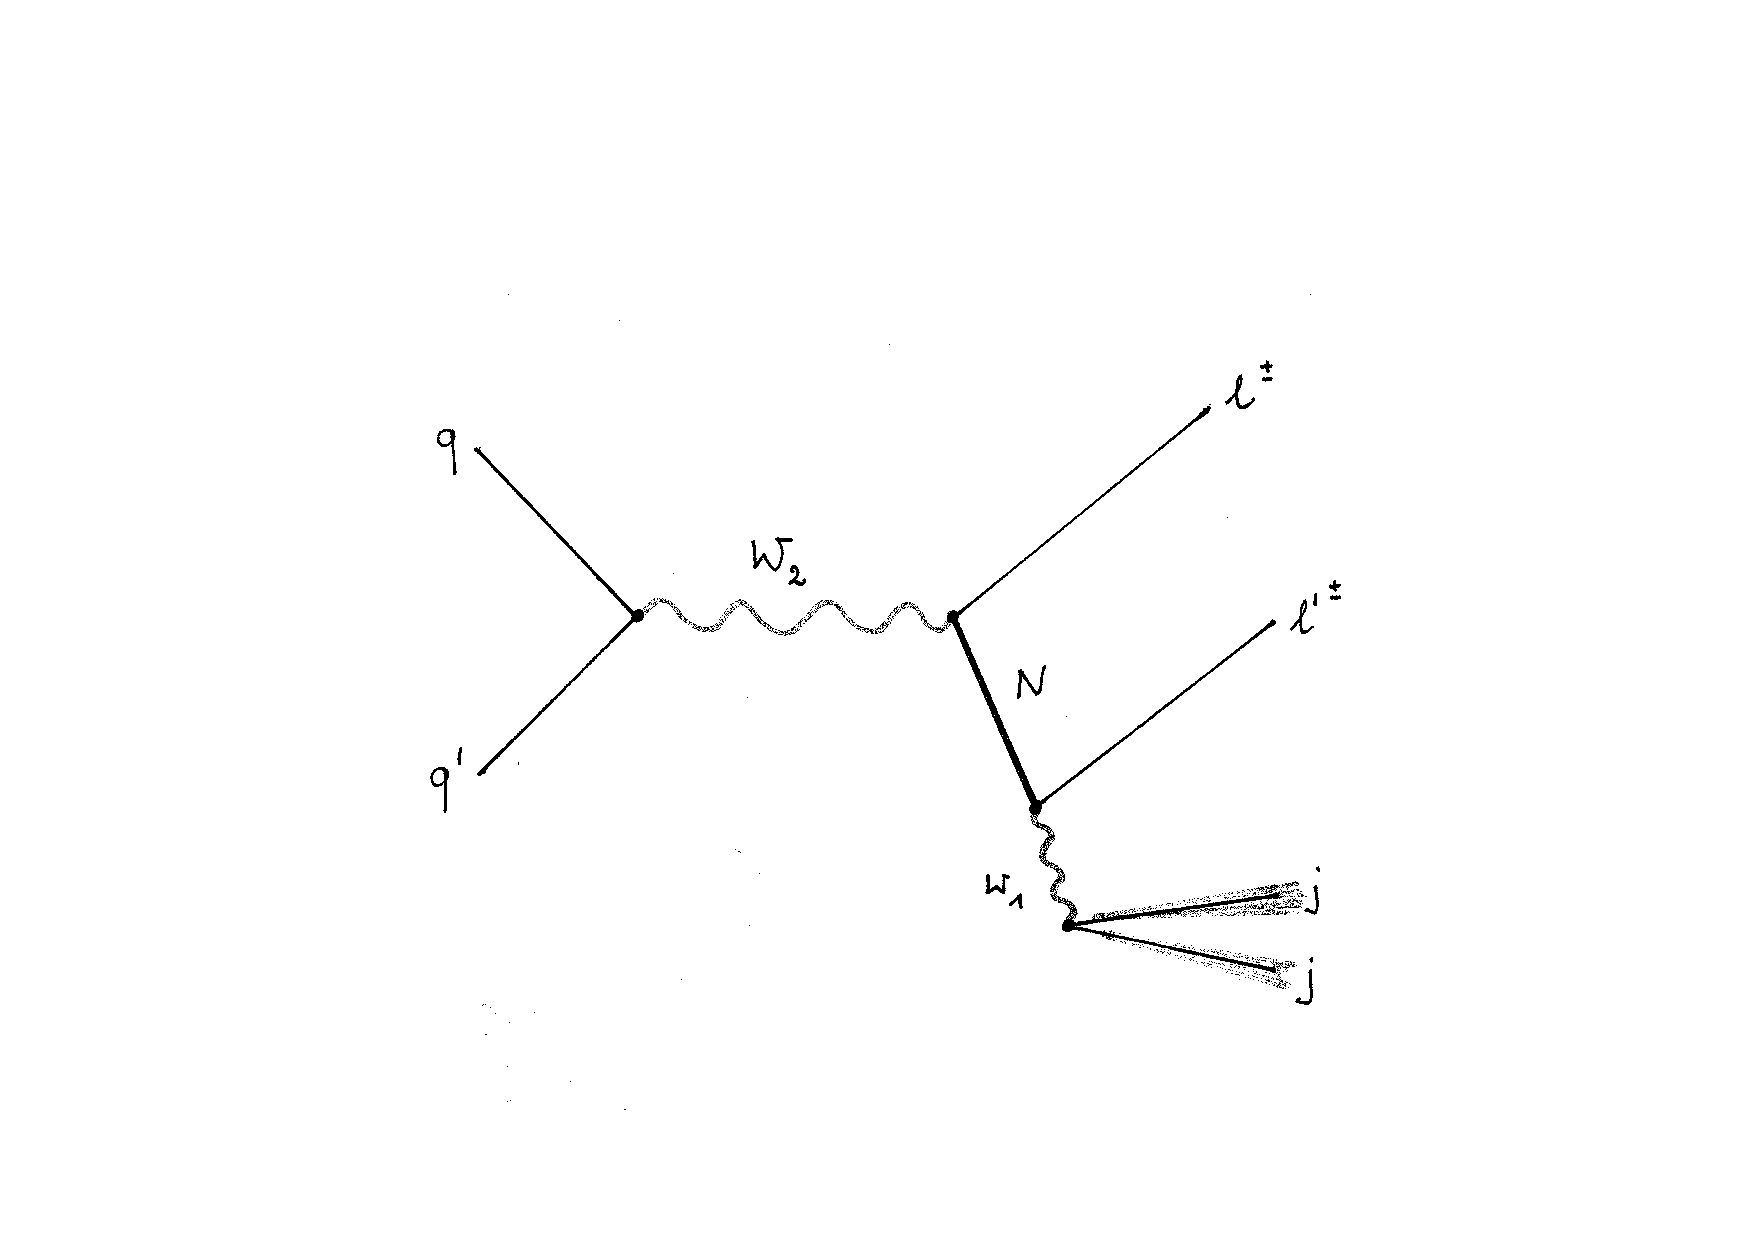
\includegraphics[scale=0.5]{pp_WR}
%\includegraphics[scale=0.5]{CMS-ppeejj-3}
\caption{ 
Production signal of a heavy gauge bosons $W_2$ decaying to charged leptons $l_i$ ($i=1,2,3$) and an on-shell heavy neutrinos $N_a$ ($a=1,2,3$).
%\cite{Keung:1983uu}. 
Heavy neutrinos further decays mainly  via 3-body process $N_a\to l_jjj$ leading to two jets and two charged leptons in the final state:
$pp\to W_2^{\pm}\to l_i^{\pm} N_a\to l_i^{\pm} l_j^{\mp}jj\; \textrm{(OS)}$
and 
$pp\to W_2^{\pm}\to l_i^{\pm} N_a\to l_i^{\pm} l_j^{\pm}jj\; \textrm{(SS)}$.
%\leavevmode\\ \begin{minipage}{\linewidth}
%\begin{eqnarray*}
%pp\to W_2^{\pm}\to l_i^{\pm} N_a\to l_i^{\pm} l_j^{\mp}jj,&&\quad\textrm{(OS)}\\
%pp\to W_2^{\pm}\to l_i^{\pm} N_a\to l_i^{\pm} l_j^{\pm}jj.&&\quad\textrm{(SS)}.
%\end{eqnarray*}
%\end{minipage}
For Majorana neutrinos, in the SS case the leptonic crossed diagram exists.
}\label{lljj}
\end{center}
\end{figure}
%Let us discuss this diagram shortly. 
This is a prominent process which has been discussed long before LHC\footnote{
Apart from this often called "smoking gun" process where heavy neutrino states can be discovered and LFV can be investigated, there are also other interesting LHC process like... considered in ....} and even Tevatron era \cite{Keung:1983uu}.
In this process same-sign (SS) leptons indicates lepton number violation, which indirectly reveals Majorana neutrino nature. If only excess is seen with opposite-sign leptons, this would indicate that Dirac neutrinos are there. In between, 
kinds of mixed states are possible. It is known from Feynman rules \cite{Gluza:1991wj,Denner:1992me} that a charged lepton determines lepton number flow in a vertex, so a neutrino is uniquely a particle or an antiparticle, depending on a sign of the charged lepton. That is why charged currents driven by charged gauge bosons or scalars can not lead to determination of neutrinos nature \cite{Gluza:1991wj}.  Neutral currents change situation but  $Z$ bosons are explicitly absent in Fig.~\ref{lljj} (for a specific contribution of Higgs bosons, see Appendix~\ref{appscal}). What remains is the Majorana propagator, which is self-conjugate.  Then on the way from one vertex to the another, 
lepton number can change, resulting in the same two final charged leptons.  

For further discussion, we  introduce three  parameters which should be fitted to the experimental data. The first parametrizes  the number of SS events  to the number of OS events\footnote{In \cite{Gluza:2015goa} mistakenly $r_{\rm{CMS}}=\frac{1}{14}$ was assumed. However, CMS estimated 13 OS events. Fortunately,  $r_{\rm{CMS}}<<1$, so this change practically does not influence  motivation, discussion and results given in \cite{Gluza:2015goa}.} 
\begin{equation}
r=\frac{ N_{SS}}{ N_{OS}},\; r_{\rm{CMS}}=\frac {1}{ 13},\label{r}
\end{equation}
 the second gives the ratio of different flavour dileptons
 \begin{equation}
r'=\frac{ N_{\mu \mu jj}}{ N_{eejj}}\label{rp},\;r'_{\rm{CMS}}=0,
\end{equation}

finally, the third parameter cares about the excees in the total cross section

\begin{equation}
\gamma=\frac{\sigma(pp\to eejj)_{CMS}-\sigma(pp\to eejj)_{SM}}{\sigma(pp\to eejj)_{0}} , \; \gamma_{\rm{CMS}}\simeq 0.54.
 \label{gamma}
\end{equation}

Index $A$ in Eq.~\ref{gamma} refers to the MLRSM cross section prediction (with $g_L =g_R$ and trivial heavy neutrino mixings and mass degeneracy, as analyzed in by the CMS collaboration)    
while $B$ refers to the cross section derived assuming $W_2$ hypothesis, see  Fig.1 for details. Such a prametrization is better for small statistics, especially in a limit of no excess, $\gamma=0$? 
 
%For Dirac neutrinos $r=0$. For Majorana neutrinos  $r=1$. What about intermediate possibilities? They are called commonly  pseudo-Dirac or quasi-Dirac neutrinos. Originally these are some special constructions of active and/or sterile neutrinos defined with specific Dirac-Majorana mass matrix relations \cite{Wolfenstein:1981kw,Bilenky:1987ty} which differs from what is usually needed in the heavy TeV neutrino case.  We will look at this case more precisely. 

%We should stress that statistically the signal is not impressive, its local significance is calculated at the 2.8 $\sigma$ level and the ATLAS does not see the same. Though, we should also stress that in ATLAS analysis the search focus on SS signals only, assuming heavy 
%Majorana nature of neutrinos. We will comment also on this strategy in a moment. 

%In the next section we will define the problem we address in the paper. Then we will c\begin{figure}[h!]

\begin{figure}
\begin{center}
%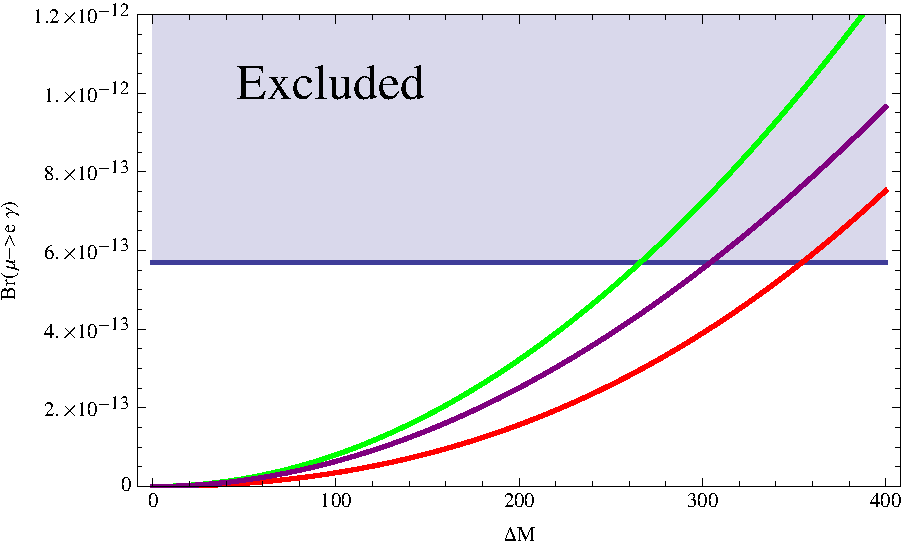
\includegraphics[scale=0.5]{Plot1}
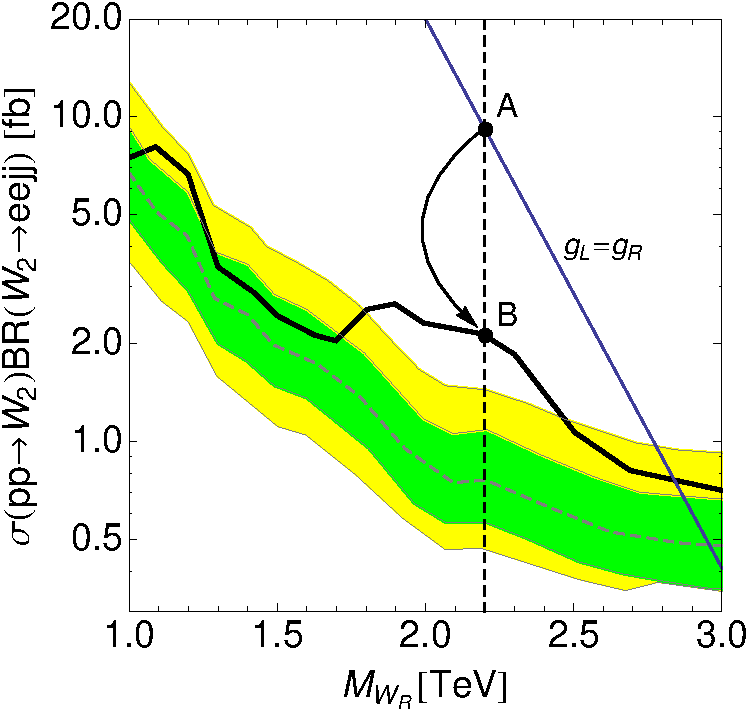
\includegraphics[scale=0.6]{CMS-ppeejj-4}
\caption{Brazil band and  Tomek, opisz A,B,C,D i odpowiednio wprowadz litery w eq.5}   \label{meg2}
\end{center}
\end{figure}
 

%\section{Influence of heavy neutrinos on the $pp\to lljj$ process.\newline
%Setting the problem with adequate questions}


%We do not try to deduce what kind of mass generation or see-saw type mechanism (type I-III, linear, inverse) are responsible for the anomaly. Rather our motivation is in a direction of the data analysis undertaken by LHC collaborations. We argues and encouarge to undertake more refine .....

Eqs.~\ref{r}-\ref{gamma} can be reconciled with Eq.\ref{lagr2} for the following neutrino mass parameters (and $M_{W_2}=2.2$ TeV) 
 
\beq
M_{N_{1,3}}=0.925\,\mathrm{TeV},\quad M_{N_2}=10\,\mathrm{TeV}
\eeq
and mixing matrix of the form:
\beq\label{KRB13}
K_{R}=
\left(
\begin{array}{ccc}
\cos\theta_{13}&0&\sin\theta_{13}\\
0&1&0\\
-e^{i\phi_3}\sin\theta_{13}&0&e^{i\phi_3}\cos\theta_{13}
\end{array}
\right),
\eeq 
\\
choosing $\theta_{13}=...$ and $\phi=/pi/2$, for details, see  \cite{Gluza:2015goa}.

Using parametrization Eq.~\ref{KRB13}, Eq.~\ref{lagr2} explicitly reads
\beq
\mathcal{L_{RHC}}=    
{\left(
 \cos \theta_{13} \overline{N}_1 - e^{i \phi_3}\sin \theta_{13} \overline{N}_3
  \right)} \Omega
% \\
%&\times& \frac{\tilde{g}}{\sqrt{2}} \gamma^{\mu}P_R(K_{R})_{aj}l_jW_{2\mu}^{+} +\mathrm{h.c.} 
\label{lagr3}
\eeq
where $\Omega =\frac{\tilde{g}}{\sqrt{2}} \gamma^{\mu}P_R(K_{R})_{aj}l_jW_{2\mu}^{+}$. 

As we can see, neutrinos $N_1$,$N_2$ contributes with different weights into vertices in Fig.~\ref{lljj}, if neutrinos are non-degenerate, additional weigth factors appears. Both neutrinos interfere leading to different values of $r$ and $\gamma$ parameters, as shown in Fig.~\ref{figr1}. Present CMS $r$ and $\gamma$ values prefer pseudo-Dirac neutrinos (for Dirac case, bottom star, mixing between two Majorana neutrino states should be maximal $\theta=\pi/4$, so the CP phase $\phi=\pi/2$). For two top stars, there is no mixing among neutrino states and neutrino is purely of Majorana neuture. In Fig.~\ref{figr1}
it is also shown what happend if masses of Majorana neutrinos are not the same, here however also Majorana decay widths are important.

\begin{figure}[h!]
\begin{center}
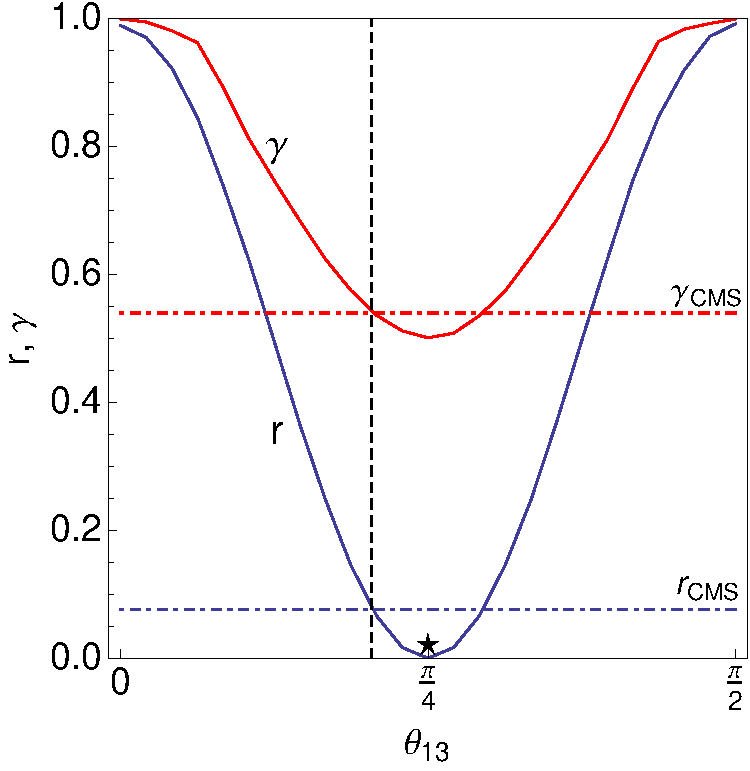
\includegraphics[scale=0.55]{splitting0GeV-2}
\caption{
TOMEK: inny rysunek, wszystko ma byc na jednym. 
Dependence of $r$ (blue) and $\gamma$ (red) on $\theta_{13}$ for $M_{N_1}=M_{N_3}=925\,\mathrm{GeV}$ and $M_{N_2}=10\,\mathrm{TeV}$. Horizontal dot-dashed lines show values of $r_{\mathrm{CMS}}=0.07$ and $\gamma_{\mathrm{CMS}}=0.54$ observed in the CMS experiment. Vertical dashed line corresponds to the value of $\theta_{13}$ for which both $r=r_{\mathrm{CMS}}$ and $\gamma=\gamma_{\mathrm{CMS}}$. A star represents a scenario in which  $\theta_{13}=\pi/4$ and $\phi_3=\pi/2$ what gives Dirac-type heavy neutrino.} \label{figr1}
\end{center}
\end{figure}
 

In the diagrams we consider the kinematics and masses of particles allows for the exchange of a neutrino close to its mass shell. Then the total cross section is dominated by the exchange of the neutrino in the s-channel. Close to the mass pole its energy dependence can be described by the Breit-Wigner type distribution. If more  than one neutrinos are presented, amplitudes corresponding to different mass eigenstates have to be added coherently. When cross section is calculated,  the interference term between different amplitudes can be negative and suppress SS lepton production. The size of the interference term can compete with the Breit-Wigner contribution only if the neutrino mass difference is of the order of the neutrinos widths (lines.... in Fig). Otherwise the interference term contributes only to the continuum background and is irrelevant for processes where the dominant contributions comes for the resonant s channel (line ...). Therefore the possible suppresion of the SS signal can occur only if the heavy Majorana neutrinos are almost degenerated. 



Based on results shown in Fig.~\ref{figr1}, different scenarios are summarized in Table

\begin{table}[h!]
%\begin{center}
\begin{tabular}{|c|c|c|c|}
\hline \hline
    $\epsilon=\frac{\Delta M}{max(\Gamma_i)}$ & 
    %$\epsilon'=\frac{\Delta M}{min(M_i)}$ & 
    %${\cal{O}}$ 
    r, Eq.3 & $\Delta L$ violation   & Nature  \\
\hline
0 & 0 & 
%0 & 
0 & Dirac \\ 
 $<< 1$ & 
 %$<< 1  $&
   small & moderate   & pseudo-Dirac  \\
  $\sim  1$ & 
  %$\leq  1$ &
   large   &  substantial & Majorana\\
  $>>1$ & 
  %$>> 1$ & 
  1 & maximal & Majorana \\
\hline \hline
\end{tabular}
%}
%\end{center}
\caption{Dirac-ness of neutrino states composed of Majorana massive states measured by $r$ parameter (Eq.\ref{r}) in $pp \to lljj$, see Fig.~\ref{figr1}.}
\end{table}

  
We may ask how to describe a situation in a case of stable neutrinos, in this case neutrino decay width is zero. We can think here about light active SM neutrinos. In this case Dirac nature of neutrinos is restored as ..... Robert....

Robert: moze lepiej?:
To make the picture complete, we can think about a situation is where a 
process is t-channel dominated and, as discussed above, neutrino decay widths are irrelavant. Here interferences can be substantial even for very large Majorana neutrino mass splittings, leading effectively to restoration of the lepton flavour (destructive interference may kill the cross section totally). This can happen for another variant of the diagram shown in Fig.\ref{figr1} in which quark and jet lines are removed: $e^-e^- \to W^-W^-$. This situation has been discussed in cite , we update it here in a different context. moze appendix nie jest potrzebny, jedynie wykres

PONIZEJ JESZCZE NIE ZROBIONE:

mu e gamma, tau e gamma bezneutrinowy


This is a simplified 


mamy tylko $L_CC$ lagrangian z mieszaniem stanu N. to wszystko. katy mieszania i masy sa input parametrami, to be fixed in experiments. Our aim is to show that taking such subtle details of the right handed sector gives a deeper insight into results, otherwise many things can be missed. One example. In the ATLAS experiment .... SS ...-> Dirac missed



% Certainly new LHC2 data running at higher energies will improve also statistics and  will be decisive. However, even if presently not established in a solid way, the situation deserves attention, also from the theoretical point of view. In fact, many analysis have been undertaken where the anomaly is analyzed
%\cite{Deppisch:2014qpa,Heikinheimo:2014tba, Deppisch:2014zta,Aguilar-Saavedra:2014ola, Ng:2015hba,Dobrescu:2015qna,Berger:2015qra,Krauss:2015nba,Brehmer:2015cia,
%Dhuria:2015swa,Dev:2015pga,Coloma:2015una}. 
%This is a prominent process which has been discussed long before LHC\footnote{
%Apart from this often called "smoking gun" process where heavy neutrino states can be discovered and lepton number violation can be investigated, there are also other interesting LHC process like... considered in ....} and even Tevatron era 
%\cite{Keung:1983uu}. We would like to clarify some issues and give  more details exploring possible neutrino effects. 
%We will follow mainly work \cite{Gluza:2015goa} where CMS data has been interpreted solely through the right handed neutrino sector connected with the pure Majorana neutrinos. In numerical analysis we use Feynrules ... and Madgraph ... where we defined self-conjugate neutrino fields, and let them go. In some works it has been noted that the specific example given in \cite{Gluza:2015goa} indicates in the direction of pseudo-Dirac neutrinos .... Independent  interpretations of the signals with help of pure Dirac neutrinos also appears .... In fact, situation is interesting and neutrino nature is one of key features which determines $r$ and $\gamma$ parameters. \\

 Common reasoning for that is the following: \\
%\begin{frame}
{\it For Majorana neutrinos the same number of SS and OS events is expected, \\
and as CMS indicates strongly that $r <<1$, then Dirac-type of neutrinos must be involved.} 
%\end{frame}

%Basically this statement is true, though it can lead to some misinterpretations.
%However,  this logic can be misleading. 
In principle, that no lepton number violation is observed does not necesserarily mean that Dirac neutrinos are there. Imagine for instance the process where only charged currents are involved. Such a situation was discussed in the introduction. On the other hand, if lepton number is violated then Majorana neutrinos are there \cite{Schechter:1981cv}.

Second remark is more important.  There are many theoretical arguments for heavy Majorana massive neutrinos: they are more economic as only two degrees of freedom are needed, they may lead altogether with small Dirac mass terms to the see-saw mechanism. So, if experimentalists would trust intuition of theoreticians and we assume that heavy Majorana neutrinos exist then to check it experimentally, enough is to find lepton number violating events, in our process these are SS dileptons. However, if no SS signals are found, then possibility that neutrinos are of Dirac type is missed. And this seems to be exactly the ATLAS collaboration case.

%czy to ma sens:
%Let us assume that we have a pure Dirac massive neutrino state.  From the theory we know that this state can be written as a composition of maximally entangled two degenerate Majorana mass states with opposite CP parities. Are they physical particles or they always act effectively as Dirac particles? If we could produce them directly in experiments, due to opposite CP parities,  their decays would be different. Situation is similar to the measurement of the longitudional polarization modes of gauge bosons at high energies, which is equivalent to scattering of Goldstone bosons.  So, it is also very important to know to which extend neutrinos are degenerate, and what is their actual superposition in terms of Majorana massive states.

Let us note that in the original paper \cite{Keung:1983uu} which is usually invoke in this situation it was really shown that for Majorana neutrinos $r=1$. However, in this paper the mixing between generations of heavy neutrinos was ignored and a simple factorization of the process into $W_R$ production times branching ratios is possible. Then, of course, number of same sign eejj events is equal to opposite sign eejj events, even for non-degenerate Majorana neutrino masses. Further rule of thumb arguments  for that are given in the Appendix. 
 
This is a mass matrix for three types of massive Majorana neutrinos with general CP phases.
%In \cite{Gluza:2015goa} 
We know elements of this matrix quite well in the light sector, it has almost tri-maximal form , meaning that mixings among $\nu_1-\nu_2$, $\nu_1-\nu_3$ and $\nu_2-\nu_3$ flavours are large. Now, what can we say about right-handed sector? It is a kind of a {\it tabula rasa}, but not completely as limits on signals driven by such heavy neutrino states exist. Presently the stringest constraint comes from the lepton flavour violating $\mu \to e \gamma$ process.	

\begin{table}[h!]
\noindent \begin{centering}
\begin{tabular}{|c|c|c|}
\hline 
Process & Current Limit & Planned Limit\tabularnewline
\hline 
\hline 
$\tau\rightarrow\mu\gamma$ & 6.8E-8 & 1.0E-9\tabularnewline
\hline 
$\tau\rightarrow\mu\mu\mu$ & 3.2E-8 & 1.0E-9\tabularnewline
\hline 
$\tau\rightarrow eee$ & 3.6E-8 & 1.0E-9\tabularnewline
\hline 
$\mu\rightarrow e\gamma$ & 5.7E-13 & 1.0E-14\tabularnewline
\hline 
$\mu N\rightarrow eN$ & 7.0E-13 & 1.0E-17\tabularnewline
\hline 
$\mu\rightarrow eee$ & 1.0E-12 & 1.0E-16\tabularnewline
\hline 
\end{tabular}
\par\end{centering}

\caption{Current and planned limits on Lepton CFLV}
\end{table}

For unitary $K_{R}$, ($\left(K_{R}^{\dagger}K_{R}\right)_{e\mu}=0$)
and for $\left(\frac{m_{i}}{m_{W_{R}}}\right)\ll1$, assuming mixing
only between two generations we get simplified equation
\begin{equation}
Br(\mu\rightarrow e\gamma)=\frac{3\alpha}{32\pi}\left(\frac{m_{W}}{m_{W_{R}}}\right)^{4}\left(\sin\theta\mbox{\ensuremath{\cos\theta}}\frac{\Delta m_{12}^{2}}{m_{W_{R}}^{2}}\right)^{2}.\label{eq:mu2egamma}
\end{equation}

For maximal mixing between two generations, $M_{W_{R}}=2200\,\mathrm{GeV}$
and neutrinos masses at the scale of TeV, we need the splitting to
be of the order of about 100GeV to get an agreement with the current
bounds, see Fig.~\ref{meg1}. In other words, the splitting must be smaller than about $100\,\mathrm{GeV}$.
The splitting depends also on the mass of the neutrino itself, as shown in Fig.~\ref{meg2}.

  {\bf Robert, dokladnie jakie parametry? opisz caption figs}
  
  \begin{figure}[h!]
  \begin{center}
  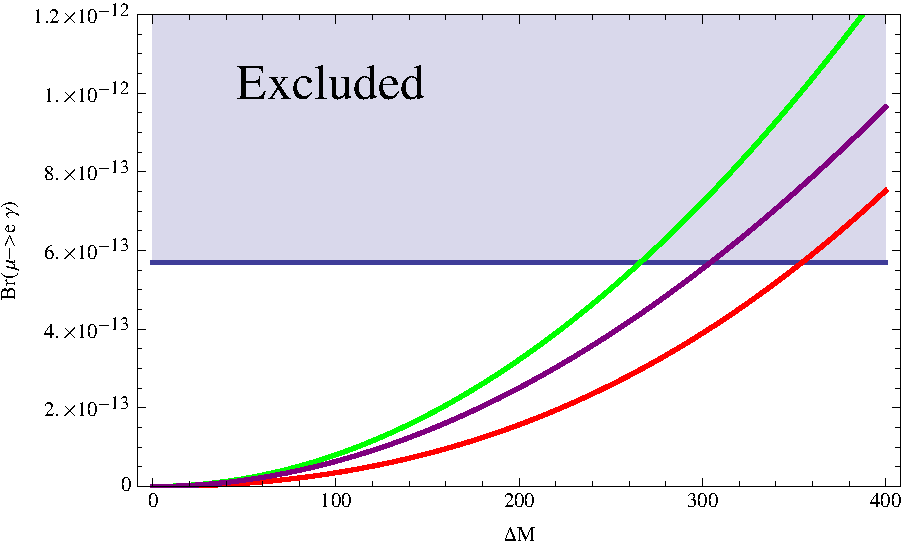
\includegraphics[scale=0.5]{Plot1}
  %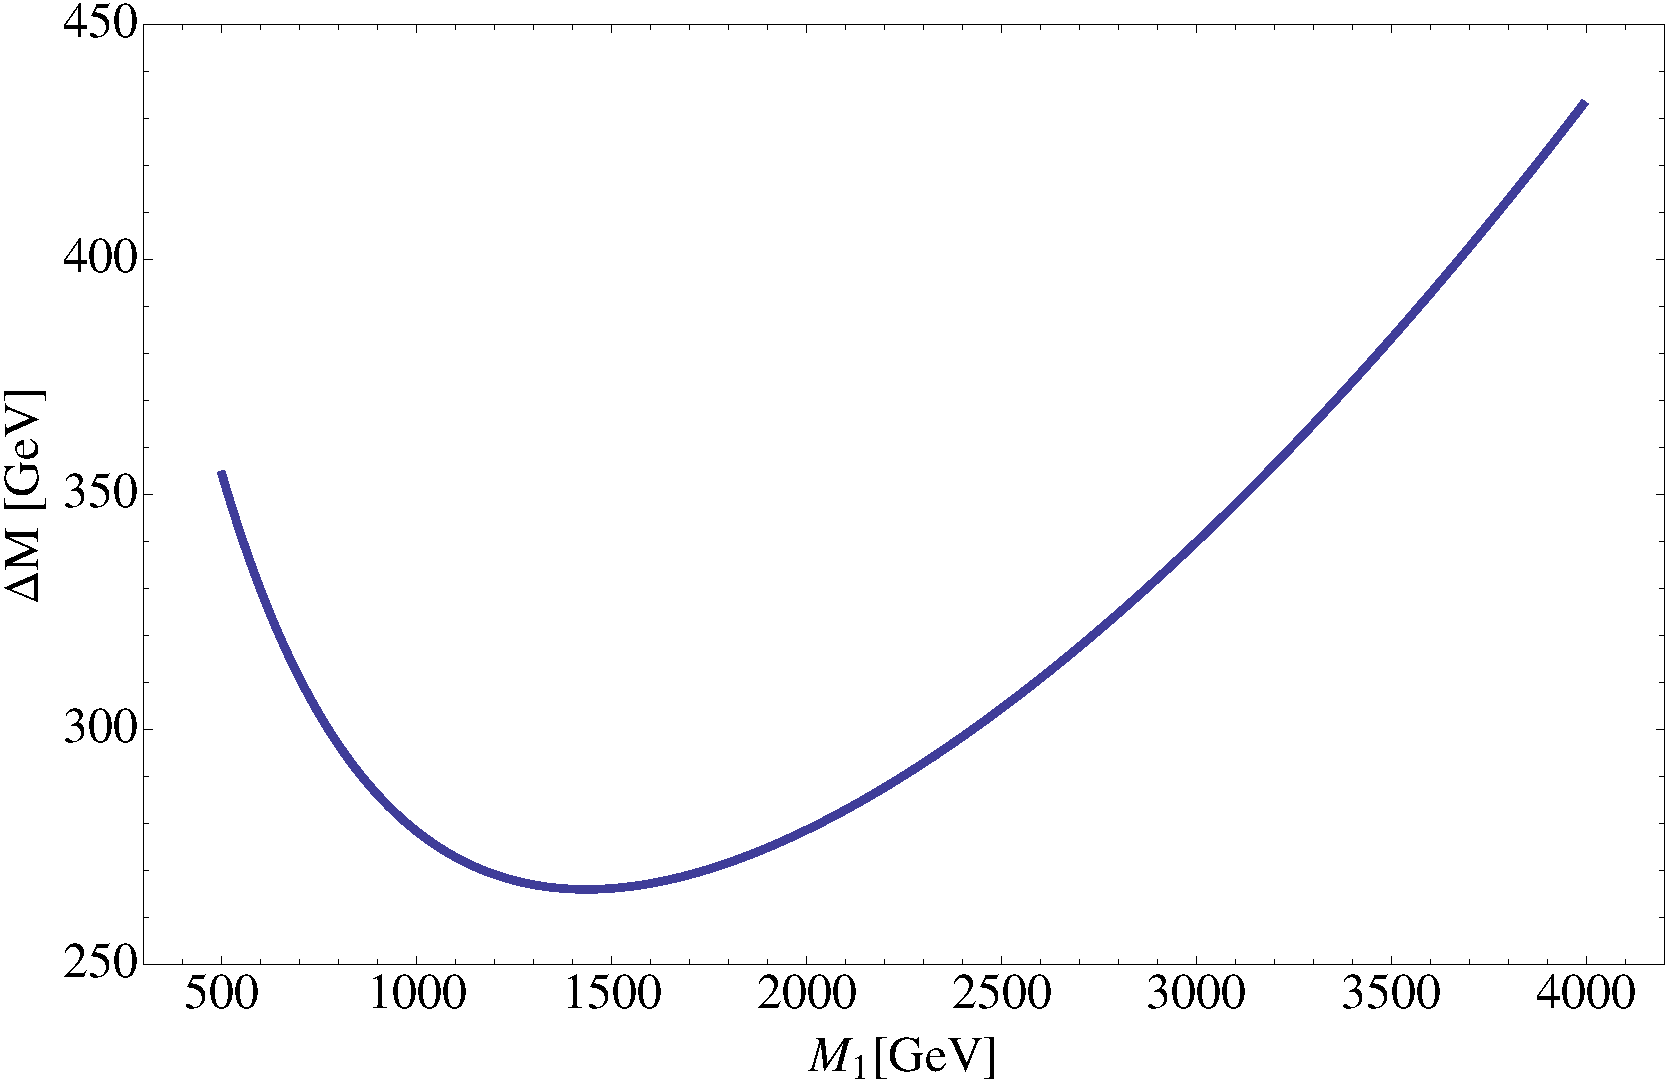
\includegraphics[scale=0.5]{Plot2}
  \caption{Estimation of the maximal splitting between heavy neutrino masses allowed for large LFV $\mu \to e \gamma$ process.   
  }
  \end{center}\label{meg1}
  \end{figure}
  


%\section{Interferences and degeneracy of Majorana neutrinos}


\begin{figure}[h!]
\begin{center}
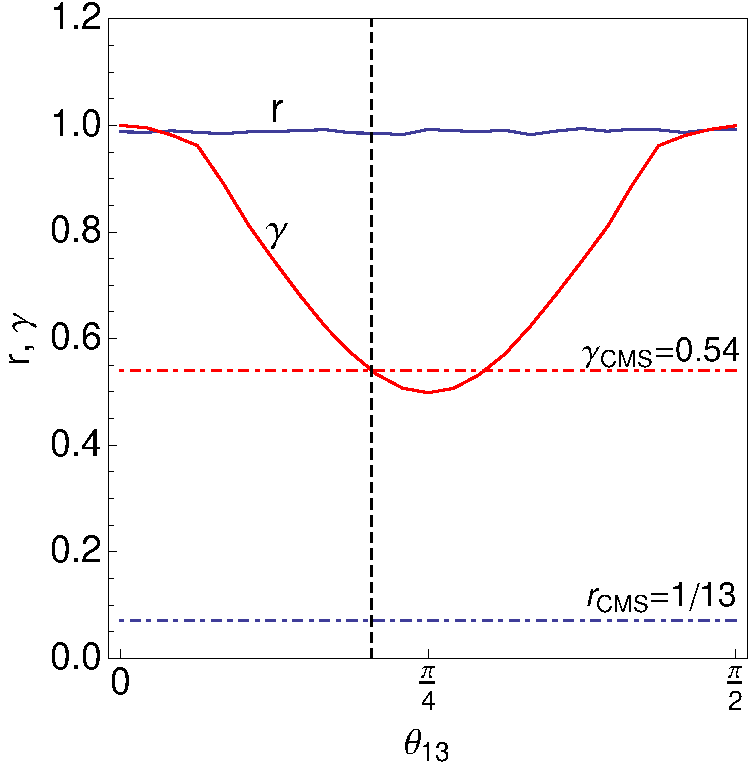
\includegraphics[scale=0.6]{splitting1GeV-3}
\caption{Dependence of $r$ (blue) and $\gamma$ (red) on $\theta_{13}$ for $M_{N_1}=924.5$, $M_{N_3}=925.5\,\mathrm{GeV}$ and $M_{N_2}=10\,\mathrm{TeV}$. Horizontal dot-dashed lines show values of $r_{\mathrm{CMS}}=0.07$ and $\gamma_{\mathrm{CMS}}=0.54$ observed in the CMS experiment. Vertical dashed line corresponds to the value of $\theta_{13}$ for which $\gamma=\gamma_{\mathrm{CMS}}$.}\label{figr2}
\end{center}
\end{figure}


Based on Figs.\ref{figr1},\ref{figr2} let us try to summarize  


pozniej...
We can also  look at this diagram different way: rotating the diagram by 90 degrees and directing the jets oppositely, we get simple the main diagram which is responsible for the neutrinoless doubly beta decay. This is why investigating  process in Fig.~\ref{lljj}, LFV low energy processes should be also considered ...ref...

%\section{Interferences and Majorana neutrino decay widths}
 

\section{Summary}
We have considered potential effects of the dileptons signals coming purely from the heavy neutrino sector, neglecting large light-heavy neutrino mixings, for which see-saw I type is not enough, and we need other modelling, for instance through inverse see-saw mechanisms \cite{}. In this case future lepton colliders would be a good place to diseantangle the models.

we discussed typical hadron, lepton and low energy processes which in fact intersect each other....

even if CMS not survice, our discussion shows possible way how....

  

\section*{Acknowledgements}

We would like to thank Marek Zra\l ek  and Dobrescu? for interesting discussions. 
%
Work is supported by the Polish National Science Centre (NCN) under the Grant Agreement No.\linebreak[4] DEC-2013/11/B/ST2/04023 and under postdoctoral grant No. DEC-2012/04/S/ST2/00003.

\section{Appendix 1. Majorana neutrinos and the  $r=1$ dileptons process \label{appdir}}

TOMEK

If we look in the basic diagram in Fig.1, we can see that the amplitude for the signal is a sum of terms from intermediate neutrino states, weighting by the neutrino mixing matrix $KR$ and kinematical factors.



In the SS case we have two $K_R$ mixing elements with the same complex conjugacy while in the OS case they are opposite, which matters for CP effects.

{\bf Tomek, jak to najlatwiej pisac prostymi wzorami?}

...

In the case non-degenerate case such simple arguments are absent and we have to make numerical estimations. 

\section{Appendix 2. MLRSM Higgs bosons contributions to the dileptons-plus-two-jets process \label{appscal}} 

%\appendix{ddddd}

MAGDA

\section{Appendix 3. Off-shell interferences of Majorana neutrinos with large mass splittings in the $e^-e^- \to W^-W^-$ process  \label{appll}}

MAGDA/TOMEK

moze niepotrzebny, tylko rysunek w glownym

\section{Appendix 4. LFV low energy processes.   \label{applfv}}

ROBERT: UPORZADKUJ, potem cos sie wrzuci do glownego, zobacz co z tau-> e gamma, czy nasze KR jest ok, no i rysunek do neutrinoless

Neglecting light-heavy neutrinos mixing, Eq.\ref{V}, branching ratio for $\mu\rightarrow e\gamma$ is \cite{Bu:2008fx}

\begin{eqnarray}
Br(\mu  \rightarrow  e\gamma) &=& 3 \frac{\alpha}{8\pi} \left(\frac{m_{W_{1}}}{m_{W_{2}}}\right)^{2}   \nonumber \\ 
&  & \left|  \sum_{i} \left(K_{R}^{}\right)_{ei}\left(K_{R}^{}\right)_{i\mu}F\left(\frac{m_{i}^{2}}{m_{W_{2}}^{2}}  \right)  \right|^{2}
\end{eqnarray}
where $m_{i}$ is the mass of the heavy neutrino and  

\begin{eqnarray}
F(x)&=&\frac{1}{6\left(1-x\right)^{4}} \nonumber \\
&\times & \left[10-43x+78x^{2}-49x^{3}+4x^{4}+18x^{3}\ln x\right].
\end{eqnarray}
%And function $G$ is 
%\[
%G(x)=\frac{1}{\left(1-x\right)^{3}}\left[-4+15x-12x^{2}+x^{3}+6x^{2}\ln x\right].
%\]

Sum over $i$ runs over all six neutrinos. Light neutrino contribution
is negligible, unless there is a large contribution due to the non
unitarity of $K_{L}$. 

For unitary $K_{R}$, ($\left(K_{R}^{\dagger}K_{R}\right)_{e\mu}=0$)
and for $\left(\frac{m_{i}}{m_{W_{R}}}\right)\ll1$, assuming mixing
only between two generations we get simplified equation
\begin{equation}
Br(\mu\rightarrow e\gamma)=\frac{3\alpha}{32\pi}\left(\frac{m_{W}}{m_{W_{R}}}\right)^{4}\left(\sin\theta\mbox{\ensuremath{\cos\theta}}\frac{\Delta m_{12}^{2}}{m_{W_{R}}^{2}}\right)^{2}.\label{eq:mu2egamma}
\end{equation}
Notice that the same equation holds also in the case of light neutrinos,
if we put $m_{W_{R}}=m_{W}$. This contribution is negligible since
\[
\frac{\Delta m_{12}^{2}}{m_{W}^{2}}\approx\frac{10^{-3}\text{{eV}}^{2}}{80\text{{GeV}}^{2}}\sim10^{-25}.
\]

For $M_{W_{R}}=2200$GeV the branching ratio is suppressed by $\frac{3\alpha}{8\pi}\left(\frac{m_{W}}{m_{W_{R}}}\right)^{4}\sim10^{-9}$,
which gives good estimation of the order of magnitude. To get an agreement
with experimental bounds we need to adjust masses and mixing, such
that $\left|\left[K_{R}^{\dagger}F\left(\frac{m_{i}^{2}}{m_{W_{R}}^{2}}\right)K_{R}\right]_{e\mu}\right|^{2}\ll1$.
For unitary $K_{R}$ the important suppression comes, not directly
from the masses of neutrinos, but rather from the splitting of the
masses. For maximal mixing between two generations, $M_{W_{R}}=2200\,\mathrm{GeV}$
and neutrinos masses at the scale of TeV, we need the splitting to
be of the order of about 100GeV to get an agreement with the current
bounds, see Fig.~\ref{meg1}. In other words, the splitting must be smaller than about $100\,\mathrm{GeV}$.
The splitting depends also on the mass of the neutrino itself, as shown in Fig.~\ref{meg2}.

  {\bf Robert, dokladnie jakie parametry? opisz caption figs}
  
  \begin{figure}[h!]
  \begin{center}
  %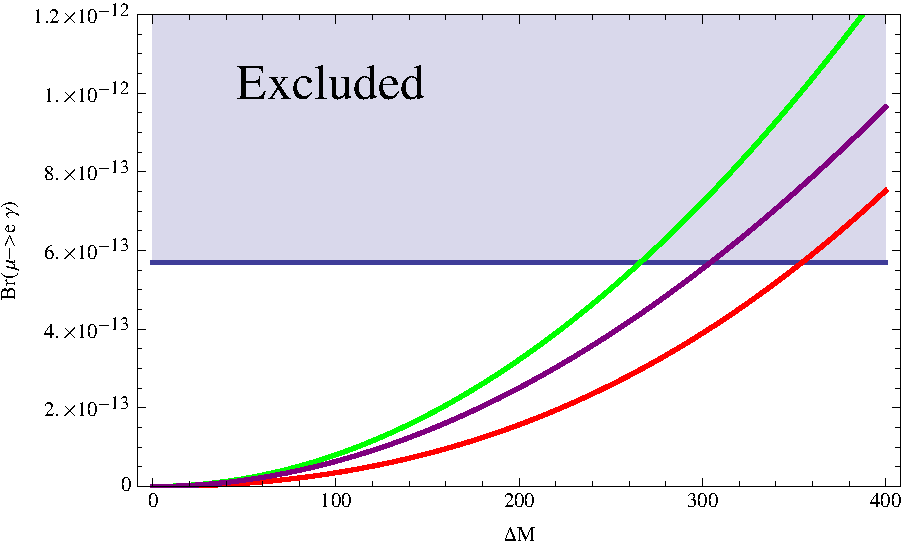
\includegraphics[scale=0.5]{Plot1}
  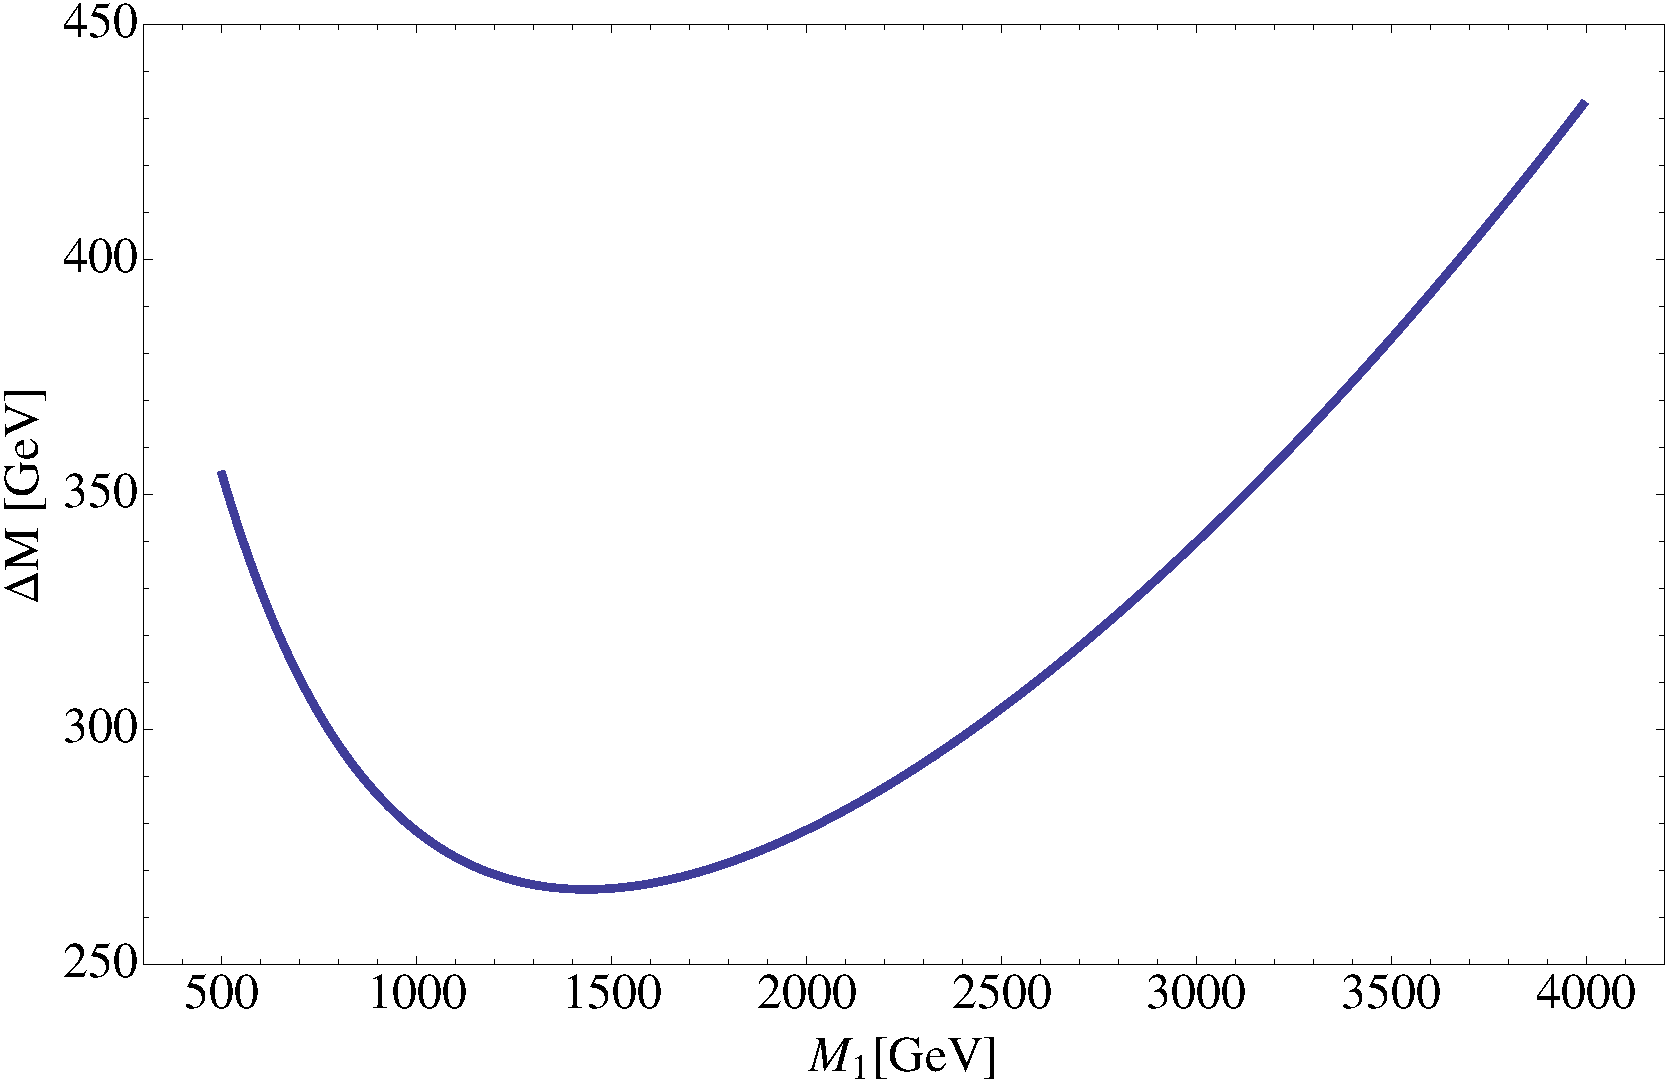
\includegraphics[scale=0.5]{Plot2}
  \caption{Estimation of the maximal splitting between heavy neutrino masses allowed for large LFV $\mu \to e \gamma$ process.   
  }
  \end{center}\label{meg2}
  \end{figure}
  

jaki wklad bezneutrinowy daje w tym przypadku? jaki wklad od lekkich?



\section{Appendix 5. In the beginning was the word: short history of neutrinos naming  \label{apphis}} 

MOJE

  Neutrinos: Dirac, pseudo-Dirac, quasi Dirac, schizophrenic, ... 
 
OGOLNIE: 
 
\begin{eqnarray}
N_\alpha &=& \Omega (\cos\theta N_1 +e^{i \phi} \sin\theta N_2 )  
\end{eqnarray} 

where $\Omega$ is a normalization factor. In our case where there is no light-heavy neutrino mixings  it is just 1.  
 
For $\theta = \Pi/4$ there is a maximal mixing between two Majorana states, if in addition $\phi = \pm \Pi/2$, Dirac neutrino state is constructed  \cite{Bilenky:1987ty}. Classically pseudo-Dirac neutrino has been introduced for light neutrinos demanding $m_D>> m_R$ in Eq.~\ref{massm}. In such a case neutrinos can mix maximally leading to the almost degenerate mass states  with opposite CP phases ...
Of course, for a typical see-saw this is not a case, and  another constructions are necessary, for instance, inverse or linear see-saw mechanisms...

Explicitly it means that

\begin{eqnarray}
N_e &=& \cos\theta_{13} N_1 +\sin\theta_{13} N_3 \\
N_\mu &=& N_2 \\
N_\tau &=& -e^{i\phi_3}\sin\theta_{13} N_1 +e^{i\phi_3}\cos\theta_{13} N_3
\end{eqnarray}

and for electrons produced in the process as shown in Fig.~\ref{lljj} two neutrino states $N_1$ and $N_3$ interfere. Chosing properly two parameters $\theta_{13}$ and $\phi_3$, $r$ and 
$\gamma$ values in Eqs.~\ref{r} and \ref{gamma} can be fixed. The result is shown in Fig.~\ref{rsdeg}.
 
In such models 
pseudo-Dirac nature of the RH
neutrinos, the ??smoking gun?? signal for type I seesaw, namely the lepton number violating
same-sign di-lepton signal [8] is absent in this case


pseudo-dirac inverse
\cite{Chen:2011hc}
\cite{Han:2006ip}
\cite{delAguila:2007em}
\cite{Mohapatra:1986aw}
nowy atlas \cite{Aad:2015xaa}

 
As we will discuss this situation more carefully in the paper, it is useful to see basic Feynman diagram for this reaction. 

.

It might well be that here a situation can be similar to some cases just described and the signal will disappear. However, the situation as it is makes a good reason and give an opportunity to look at the neutrino physics yet from another angle. 

  

\section{Appendix}

TEGO NIE BEDZIE

Having in mind the previous work \cite{Gluza:2015goa} and some further interesting discussions especially given in  \cite{Dobrescu:2015qna,Brehmer:2015cia,Coloma:2015una,Dev:2015pga}, we would like to answer in the present work to some  questions concerning detection of heavy neutrinos through the dilepton signals at the LHC, namely  
%As already mentioned, it well might be that the signal can dissolve with time, nonetheless,  So, the main questions which we arise are

\begin{itemize}
\item[(i)] What is an effective composition of the degenerate Majorana states which may lead
to some nonzero but small $r$, negligible $r'$ and substantial $\gamma$ parameters?
\item[(ii)] What can be the largest mass splitting among heavy neutrino states?
\item[(iii)] How heavy Majorana neutrino decay width modulates the signal?
\item[(iv)] How lepton flavour violating processes restrict right-handed neutrino mass and mixing matrices?
\item[(v)] How does departure from the $g_L=g_R$ case influence heavy neutrino sector parametrization?
\item[(vi)] Do Higgs bosons effects can be substantial?
\end{itemize}

%Our discussion is general enough to look into the problem of heavy neutrino states identification at hadron colliders from a different point of view.
Trying to answer to these general questions, we will use values of parameters connected with the CMS dilepton anomaly, Eqs.~\ref{r}-\ref{gamma}. 

%Now we come to the discussion of the neutrino sector structure driven by eqs.~(\ref{massm},%\ref{V})  and their
%consequences for the possible dilepton-plus-two-jets cross sections. 

Neutrino masses and mixings depends on the structure of the neutrino mass matrix 
\cite{Bilenky:1987ty}. As in \cite{Gluza:2015goa}, we assume a typical see-saw typy I mass matrix

\begin{equation}
M_{\nu}=\left(
\begin{array}{cc}
0 & M_D\\
M_D^T & M_R
\end{array}\right). \label{massm}
\end{equation}


We assume $M_D [{\cal{O}}(MeV)] \ll M_R [{\cal{O}}(TeV)]$ and  no light-heavy neutrino mixings

FOOTNOTE
In our typical see-saw mechanism with natural scales assumed, these mixings must be anyway small \cite{Gluza:2002vs,Chen:2011hc}.... Large light-heavy neutrino mixings can be obtained through so-called modified or inverse see-saw mechanisms \cite{Mohapatra:1986aw,Chen:2013foz,Deppisch:2015cua}.  Here typical mass matrix 
\begin{eqnarray}
        M_N  =  
 \left( \begin{matrix}
    0              & m_D         & m_L\\
                m^T_D        & 0           & M \\
                m^T_L      & M^T   & \mu_S
        \end{matrix} \right)
\label{eq:mtot}       
\end{eqnarray}
leads to the pseudo-Dirac neutrino states.
%}


In this way most of possible connections between heavy and light neutrino sectors are cut away, and we can explore heavy sector effects exclusively.
The neutrino mixing matrix takes then the following form  \cite{Gluza:2015goa}  
\begin{eqnarray}\label{V}
U\approx\left(
\begin{array}{cc}
%K_{LA}^T\approx
1 
& 
%K_{LB}^T\approx
0\\
%K_{RA}^\dag\approx
0 & K_{R}^\dag
\end{array}\right),
\end{eqnarray}
where, $K_{R}$ is an unitary $3\times3$ matrix defined by $M_R=K_{R}^T\mathrm{diag}(M_{N_1},M_{N_2},M_{N_3})K_{R}$, $M_{N_a}>0$.  

In general, $K_R$ can be parametrized \cite{Agashe:2014kda}
%Gluza:2001de,Dziewit:2011pd
in the following way
%$K_{R}=U_1UU_2$,
\beqa\label{KR}
K_{R}=U_1UU_2, 
\eeqa
where $U_1=\mathrm{diag}(1,e^{i(\alpha_{23}-\alpha_{13})},e^{i(\alpha_{33}-\alpha_{13})})$ 
and \\
$U_2=\mathrm{diag}(e^{i\alpha_{11}},e^{i\alpha_{12}},e^{i\alpha_{13}})$ while
%\begin{widetext}
\begin{equation}
U=\left(
\begin{array}{ccc}
c_{12}c_{13}&s_{12}c_{13}&s_{13}e^{-i\delta}\\
-s_{12}c_{23}-c_{12}s_{23}s_{13}e^{i\delta}&c_{12}c_{23}-s_{12}s_{23}s_{13}e^{i\delta}&s_{23}c_{13}\\
s_{12}s_{23}-c_{12}c_{23}s_{13}e^{i\delta}&-c_{12}s_{23}-s_{12}c_{23}s_{13}e^{i\delta}&c_{23}c_{13}
\end{array}
\right) \label{3times3}
\end{equation}
%\end{widetext}
and $c_{rs}$, $s_{rs}$ stand for $\cos\theta_{rs}$ and $\sin\theta_{rs}$ respectively. 


\providecommand{\href}[2]{#2}
%\bibliographystyle{utphys_spires}
\bibliography{LRref}

\end{document}





LHC is a perfect laboratory to test Beyond Standard Model (BSM) scenarios. Recently, the CMS Collaboration announced an interesting 
%yet statistically not significant, 
excess in  data, see point B on Fig. \ref{CMS}. This point is related to the process $pp\to eejj$ collected by $\sqrt{s}=8\,\mathrm{TeV}$ LHC corresponding to an integrated luminosity $19.7$ $\mathrm{fb}^{-1}$ \cite{Khachatryan:2014dka}.
Several analyses \cite{Deppisch:2014qpa, Heikinheimo:2014tba, Deppisch:2014zta,Aguilar-Saavedra:2014ola} showed that this excess can be interpreted as a signal of charged gauge boson $W_2^\pm$ with mass about $2.2\,\mathrm{TeV}$  in the Left-Right symmetric model \cite{Mohapatra:1974gc,Senjanovic:1975rk,Mohapatra:1980yp}. It is possible when gauge couplings connected with left and right $SU(2)$ groups  are not equal to each other. For a case $g_L=g_R$ see point A on Fig.~\ref{CMS} (the measured cross section is suppressed by a factor of $\gamma_{CMS}=0.23$ when compared with scenario in which $g_L=g_R$).  
Moreover,  the number of events with same-sign (SS) leptons to the number of events with opposite-sign (OS) leptons is 
\begin{equation}
r=\frac{ N_{SS}}{ N_{OS}}=\frac{1}{14},\label{r}
\end{equation}
 and, finally, no excess in $\mu\mu$ channel has been reported \cite{Khachatryan:2014dka,Khachatryan:2015gha}. 
 
Theoretical analyses of the left-right symmetric models speeded up considerable in recent years  
\cite{Maiezza:2010ic,Tello:2010am,Nemevsek:2011hz,Nemevsek:2012cd,Das:2012ii,Adelman:2012py,
Nemevsek:2012iq,Dev:2013oxa,Mohapatra:2013cia,Chen:2013foz,
Bertolini:2014sua,Maiezza:2014ala,
Vasquez:2014mxa,Aydemir:2014ama,Staub:2014pca,Dutta:2014dba,
Mahajan:2014nca,deAnda:2014dba,Senjanovic:2014pva,Maiezza:2015lza, Dev:2015vra,Senjanovic:2015yea,Bambhaniya:2013wza}, after the LHC has started its operation. It is not surprising as this collider is operating at   highest available so far energies, 
%comparing to previous machines
which means that new states of matter or new interactions can be probed more effectively.  For instance, the left-right symmetric models offer an elegant, dynamical explanation for suppression of right handed currents at low energies, and it might be that finally LHC can see them directly in experimental data analyses.\footnote{For other relevant arguments in favor of left-right symmetry, see e.g. \cite{Mohapatra:1986uf}.}

 Discovery of right-handed currents and new elementary states of matter in
form of a
charged heavy gauge boson and heavy neutrinos would be of paramount importance for our understanding of Physics in microscale.
It would also impact Physics in macroscale. For instance, details of leptogenesis depend on CP phases of decaying particles, or Big Bang Nucleosynthesis and the dark matter problem raise
questions about the matter content of the Universe \cite{unbound,Giunti:2007ry} (neutrinos may be responsible  for the matter-dominated flat Universe in which we live).
 

In this paper, we show how including details of heavy neutrinos mass spectrum, their CP phases and 
%heavy neutrino 
non-trivial mixing matrix can change a picture, leading to natural interpretation of the data within MLRSM, with $g_L = g_R$ and relatively light $W_2^\pm$ charged gauge boson mass.\footnote{In this work, we do not discuss which scenarios are more natural, those with $g_L=g_R$, or those without it. If we demand strict unification of gauge couplings then scenarios with $g_L \neq g_R$ seem to be more appropriate \cite{Deppisch:2014qpa,Heikinheimo:2014tba,Deppisch:2014zta}. However, also such models need additional modifications, like new intermediate scales or symmetries. This problem  is not of the main importance for our work, and we shall remain with the simplest possibility, which is $g_L=g_R$. MLRSM has an additional advantage as $g_L=g_R$ preserves $P$ symmetry and simplifies model parameters, e.g. gauge bosons mass relations.} In other words, we can get down from  point A to point B on Fig. \ref{CMS}, while holding $g_L=g_R$. We can also accommodate value of $r$ in (\ref{r}) and explain a shortage of muon pairs.  
%An example is specific, but conclusions which we can derive are more general.
% Namely, considering MLRSM example, we want to point out that 
%details on interference effects connected with splitting of heavy neutrino masses, non-%diagonal couplings 
%of heavy neutrinos to $W_2$ and charged leptons or CP phases of heavy neutrinos, all of them are important for interpreting experimental data, 
%An example is specific, but conclusions which we can derive are more general
%as heavy neutrinos are present within many BSM models. 
 

  


\section{Heavy neutrino interactions  and their CP parities}
We work within the MLRSM model in which $g_L=g_R$, $v_L=0$ and $\kappa_2=0$ (what results in no $W_L-W_R$ mixing). 
%parameter $\xi=0$). 
%
The scale of breaking $SU(2)_R$ is set to 
%
$v_R=4.77\,\mathrm{TeV}$,
%$v_R=5.2\,\mathrm{TeV}$, 
%
such that the mass of $W_2$ is about $2.2\,\mathrm{TeV}$ (see Fig.~\ref{CMS}).
%such that the mass of $W_2$ is about $2.4$ TeV. 
%{\bf Setting $M_N=M_{W_2}/2=1.1\,\mathrm{TeV}$ could be also in order to directly address CMS analysis.} 
%
Moreover, to simplify our considerations, let us assume that the scalar potential parameters are chosen such that all scalar particles beside the lightest Higgs boson have masses of order $v_R$. We leave discussion of their influence on $pp\to lljj$ for future studies. 

Neutrino mass matrix is chosen to be of the form
\begin{equation}
M_{\nu}=\left(
\begin{array}{cc}
0 & M_D\\
M_D^T & M_R
\end{array}\right). \label{massm}
\end{equation}
Typically, Dirac masses $M_D$ are much smaller than Majorana masses $M_R$ i.e. $M_D\ll M_R$, e.g. $M_D\sim10^{-3}\,\textrm{GeV}$, $M_R\sim10^3\,\textrm{GeV}$. Hence light neutrinos $\nu_{1,2,3}$ obtain masses $M_{\nu_{1,2,3}}$ of the order of $1\,\textrm{eV}$ via type I see-saw  mechanism. Unitary matrix $U$ which enters Takagi decomposition $M_{\nu}=U^T\mathrm{diag}(M_{\nu_1},M_{\nu_2},M_{\nu_3},M_{N_1},M_{N_2},M_{N_3})U^\dag$ is of the following form:
\begin{eqnarray}\label{V}
U\approx\left(
\begin{array}{cc}
%K_{LA}^T\approx
1 
& 
%K_{LB}^T\approx
0\\
%K_{RA}^\dag\approx
0 & K_{R}^\dag
\end{array}\right),
\end{eqnarray}
where, $K_{R}$ is an unitary $3\times3$ matrix defined by $M_R=K_{R}^T\mathrm{diag}(M_{N_1},M_{N_2},M_{N_3})K_{R}$, $M_{N_a}>0$. 
For simplicity, we assume no light-heavy neutrino mixings (they are negligible or very small \cite{seesaw}). 
Such choice of $U$ means that $W_2^\pm$ does not couple to light neutrinos $\nu_a$, and heavy neutrinos $N_a$ do not couple to $W_1^{\pm}$. Exact neutrino mixing matrix $U$ can also be considered, which include non-zero off-diagonal light-heavy matrix elements in \eqref{V} \cite{Chen:2013foz}. 

$K_R$ matrix enters directly heavy neutrinos - $W_2$ interactions, which can be cast in the following form \cite{Gluza:1993gf}:
\begin{eqnarray}
\mathcal{L}&\supset&\frac{g_L}{\sqrt{2}}\overline{N}_a\gamma^{\mu}P_R(K_{R})_{aj}l_jW_{2\mu}^{+}
%\cos\xi
+\mathrm{h.c.}\label{lagr1}
%\\
%&&-\frac{g_L}{\sqrt{2}}\overline{N}_a\gamma^{\mu}P_R(K_{R})_{aj}l_jW_{1\mu}^{+}\sin\xi+\mathrm{h.c}.
%
%\label{lagr3}\\
%
%&&+\frac{g_L}{\sqrt{2}}\overline{l}_iP_-\gamma^{\mu}
%%\underbrace{
%(K_{R})_{bi}^*
%%}_{(K_{R}^\dag)_{ib}}
%N_bW_{2\mu}^{-}\,.\label{lagr2}
\end{eqnarray}
%We set $\xi=0$ hence the second term is not relevant for the discussed setup. 

In general elements of the $K_R$ matrix can be complex. In a CP-conserving case, 
CP parities of heavy neutrinos are purely imaginary \cite{Bilenky:1987ty,cpph} and, in fact, 
%CP parities of heavy neutrinos 
they can be connected with elements of the $K_R$ matrix.
In practice, if CP parities of all three heavy neutrinos are the same, 
$\eta_{CP}(N_1)=\eta_{CP}(N_2)=\eta_{CP}(N_3)=+i$, then elements of the $K_R$ matrix can all be made real. If, for instance,  $\eta_{CP}(N_1)=\eta_{CP}(N_2)=-\eta_{CP}(N_3)=+i$ then ${K_R}_{i3}$ element is complex. 
%For general discussions including also CP-violating cases, see \cite{cpph}.
Choosing different scenarios have  far-reaching consequences in phenomenological studies.
Let us consider processes where heavy neutrinos propagate as virtual states, then their contributions to the amplitudes must be summed over. In general, 
constructive or destructive interferences between heavy neutrinos can appear. For instance, in the neutrinoless double beta decay $(\beta \beta)_{0\nu}$ process, or its inverse collider version process $e^-e^- \to W^-W^-$, 
amplitudes include squared matrix elements ${(K_R)}^2_{1a}$.   
If all heavy neutrinos have the same CP parities, then elements of the $K_R$ matrix can be made all real, and all heavy neutrinos contribute constructively into the amplitudes, otherwise  destructive interferences can appear. Such scenarios have been considered in full details in phenomenological analyses in \cite{mycp}. 
It has been shown there that cancellations among contributions to the amplitude
from heavy neutrinos with opposite CP parities can appear.  In this way, low energy $(\beta \beta)_{0\nu}$ constraints  can be avoided and  for instance the collider signal $e^-e^- \to W^-W^-$ can be substantial. 
We will see in the next Section that CP phases of heavy neutrinos play a crucial role also in a case of SS and OS $pp \to lljj$ signals.

\section{Cross sections}

We shall show that interference effects, CP phases of heavy neutrinos and their mass splittings are relevant for the prediction of the $pp\to lljj$ cross section. 
%
%To expose interference effects in a clear way, the following three different setups will be discussed: (A) neutrinos have %degenerate masses, (B) there is only small mass splitting and (C) only one of them is lighter than $W_2$. The %numerical analysis has been done with the help of \texttt{MadGraph5} (v2.2.2). 
%
%
To expose interference effects in a clear way, the following three different setups will be discussed: (A) neutrinos have degenerate masses, (B) one neutrino is lighter than $W_2$, (C) two neutrinos are lighter than $W_2$,  and, (D) finally, there is only small mass splitting among neutrinos. The numerical analysis has been done with the help of \textsc{MadGraph5} (v2.2.2) \cite{Alwall:2011uj} and with our implementation of the MLRSM in \textsc{FeynRules} (v2.0.31) \cite{Christensen:2008py,Degrande:2011ua}. 


To simplify notation we shall denote cross-sections for the process $pp\to l_i^{\pm}l_j^{\mp}jj$ by $\sigma_{l_il_j}^{\pm\mp}$ etc. For reference points it is assumed, as in CMS \cite{Khachatryan:2014dka} analysis, that $M_N=M_{W_2}/2$ with diagonal and real $K_R$ mixing matrix in (\ref{lagr1}),
%(\ref{lagr2}), 
which for 
$\sqrt{s}=8\,\mathrm{TeV}$ and  
%$v_R=4.77
%\,(5.21)
%\,\mathrm{TeV}$, 
%what gives 
$M_{W_2}=2.2
%\,(2.4)
\,\mathrm{TeV}$, gives:
\beqa\label{ppW2}
%\sigma(\texttt{\small p p > w2$\pm$})
\sigma(p p \to  W_2^\pm)
=\left\lbrace
\begin{array}{l}
71.16
%\,(36.32)
\,\mathrm{fb},\\
21.09
%\,(10.5)
\,\mathrm{fb},
\end{array}
\right.
\eeqa
what agrees with recent estimations on $pp\to W_2\to jj$ cross section \cite{Aad:2014aqa}. For chosen value of $v_R$ and diagonal matrix $K_R$ relevant branching ratios are:
\beqa
%\label{BRdeg}
\mathrm{BR}(W_2^\pm\to e^\pm N_a)=0.058,\label{BRWdeg}
\eeqa
\beqa
\mathrm{BR}(N_a\to e^\pm jj)=0.35\label{BRNdeg}
\eeqa
when all heavy neutrinos have the same mass $M_N=M_{W_2}/2$, and
\beqa
\mathrm{BR}(W_2^\pm\to e^\pm N_1) =0.066
\eeqa
when only $M_{N_1}=M_{W_2}/2$ while $M_{N_{2,3}}$ are heavier than $W_2$. 

\subsection{Degenerate masses of heavy neutrinos
%$M_{N_J}<M_{W_2}$
}

First, let us examine the following mass pattern 
%with degenerate $M_{N_J}=M_N$. 
%First, we shall consider a setup 
in which all heavy neutrinos are degenerate and lighter than $W_2$: 
\begin{equation}
M_N:=M_{N_a}=M_{W_2}/2. 
%< M_{W_2} 
\end{equation}
In this setup, and also  for small mass differences between heavy neutrinos, the narrow width approximation (NWA) will not work because of the interference effects.  
%[E. Fuchs, Cargese2014 talk]
%We want to show what can be the possible source of discrepancy between $\sigma^{\pm\mp}$ and $\sigma^{\pm\pm}$. We start from standard and general  parametrization for $K_R$, analogous as for unitary $3\times 3$ light neutrino mixing matrix, its general form is given in (\ref{3times3}). It can be done so, as we assume the complete $6\times 6$ mixing matrix in diagonal block form, see (\ref{V}). To this end, we shall 

Let us take $K_{R}$ in the following form (which is in fact a product of real, orthogonal transformation and diagonal phase matrix) 
%\cite{Bilenky:1987ty,cpph,mycp}
%
%(which is 
%explicit embedding of $U(1)\times U(2)\subset U(3)$ and 
%the most general form of mixing matrix in the case when the heaviest neutrino $N_3$ interact only with $\tau$)
\beq\label{KRB22}
K_{R}=
%e^{i\alpha_{11}}
\left(
\begin{array}{ccc}
\cos\theta_{12}&
%e^{i\gamma}
\sin\theta_{12}&0\\
-e^{i\phi_2}\sin\theta_{12}&e^{i
%(
%\gamma+
\phi_2
%)
}\cos\theta_{12}&0\\
0&0&1
\end{array}
\right).
\eeq 
%$\gamma=\alpha_{12}-\alpha_{11}$ \textbf{does not appear in the cross-section hence can be set to 0 ?}, while  
This is a simplified version of a complete unitary rotation matrix \cite{Maki:1962mu}.  
%\cite{Bilenky:1987ty,cpph,mycp}, which is given in the Appendix, (\ref{3times3}).

In this way, we assume mixings between two lepton flavors only. 
Phase 
$\phi_2
%=\alpha_{23}-\alpha_{13}
$ is connected with CP parity of heavy neutrinos $N_{1,2}$, CP-conserving case is realized when $\phi_2=0, \pm \pi/2, \pm \pi$. 
All phases which do not fulfill the above relations break CP symmetry. In general, in the MLRSM with the mass matrix of the form (\ref{massm}) we have six CP phases; if  $v_L \neq 0$ $(M_L\neq 0)$ then there are 18 CP phases \cite{aq}.

Using this simple form of the matrix $K_R$ we are already able to discuss all relevant effects connected with mixings and CP phases in the considered process.
  
%There are simple consequences of choosing~\eqref{KRB22}. 

First, in the case of degenerate neutrinos, 
$\sigma_{l_il_j}^{\pm\mp}$ with $i=j$ does not depend on mixing angles at all, and is zero for $i\neq j$:
\beqa
\label{deltaij}
%\sigma_{i-j+}&=&\\
\sigma^{\pm\mp}_{l_il_j}&=&\frac{g_L^4}{4}
%\\
%&&\times
\left|\sum_{a}F^{\pm\mp}(s,M_{W_2}^2,M_N^2)(K_{R}^\dag)_{ia}(K_{R})_{aj}\right|^2 \nonumber \\
&=&\delta_{ij}\frac{g_L^4}{4}F^{\pm\mp}(s,M_{W_2}^2,M_N^2)=\delta_{ij}\widehat{\sigma}_{SF}^{\pm\mp},
\eeqa
where the second equality comes from the unitarity of the $K_{R}$, while the third defines $\widehat{\sigma}_{SF}^{\pm\mp}$. $F^{\pm\mp}$ is a function of center of mass energy $\sqrt{s}$ and masses $M_{W_2}$ and $M_N$ (leptons and constituents of jets are treated as massless). 
%
From now on we will not write down arguments of the $F$ functions. 
%
%Note that the presence of events with $e^+\mu^-$ and $e^-\mu^+$ in the final state identified as coming from $W_2$ and degenerate $N_J$ decays will signal %that $K_{R}$ is not an unitary matrix {\bf ??? na pewno? zobacz uwage po (12)}, what is, in general, possible but needs non-zero off-diagonal parts of \eqref{V}.  

On the other hand, for same-sign signature i.e. $l^+l^+$ or $l^-l^-$ the mixing matrix $K_{R}$ does not cancel from the cross section formula: 
\beqa
\sigma_{l_il_j}^{\pm\pm}&=&\frac{g_L^4}{4}\left[F^{\pm\pm}_{1}+(-1)^{\delta_{ij}}F^{\pm\pm}_{2}\right]\nonumber\\
&&\times \left|\sum_{a}(K_{R}^\dag)_{ia}(K_{R}^*)_{aj}\right|^2.
\eeqa
%where $F^{\pm\pm}_{1,2}$ are functions of $s$, $M_{W_2}^2$ and $M_N^2$. 
As a consequence, cross section for 
$l_i^{\pm}l_j^{\pm}$ with $i=j$ is correlated with that for which $i\neq j$ i.e. 
\beqa\label{sigmaApmpm}
\sigma_{l_il_j}^{\pm\pm}&=&\left\lbrace
\begin{array}{lcc}
%\sigma_{SF}|\cos^2\theta_{12}+e^{\pm2i\phi}\sin^2\theta_{12}|^2\\
%&&=
\widehat{\sigma}_{SF}^{\pm\pm}(1-\sin^22\theta_{12}\sin^2\phi_2)&\textrm{for}&i=j,\\[1.5\baselineskip]
%&&\\
%\sigma(l_i^{\pm}l_j^{\pm})&=&
\widehat{\sigma}_{DF}^{\pm\pm}\sin^22\theta_{12}\sin^2\phi_2&\textrm{for}&i\neq j,
\end{array}\right.
\eeqa
where $\widehat{\sigma}_{SF}^{\pm\pm}$ and $\widehat{\sigma}_{DF}^{\pm\pm}$ correspond to 
%`no mixing' and `zero CP phases' scenario
maximal values of cross sections
%
for same-flavour (SF) and different flavour (DF) cases. For the numerical results see Fig. \ref{sigmaA}. 
%
 
The difference in $\widehat{\sigma}_{DF}^{\pm\pm}$ and $\widehat{\sigma}_{SF}^{\pm\pm}$ is related to the standard factor of $(-1)$ appearing in same-flavor Feynman diagrams.  For $\sqrt{s}=8\,\mathrm{TeV}$ and $M_N=1.1\,\mathrm{TeV}$ they read $\widehat{\sigma}_{SF}^{++}=1.31\,\mathrm{fb}$, $\widehat{\sigma}_{SF}^{--}=0.39\,\mathrm{fb}$, $\widehat{\sigma}_{DF}^{++}=2.61\,\mathrm{fb}$, $\widehat{\sigma}_{DF}^{--}=0.78\,\mathrm{fb}$ and $\widehat{\sigma}^{\pm\mp}_{SF}=1.70\,\mathrm{fb}$. $\widehat{\sigma}^{--}$ is about 3.4 times smaller than $\widehat{\sigma}^{++}$ due to asymmetry in production of $W_2^\pm$, see \eqref{ppW2}. 

As one can see from \eqref{sigmaApmpm} and Fig. \ref{sigmaA}, there exists a CP phase for which $(\sigma_{ee}^{++}+\sigma_{ee}^{--})/\sigma_{ee}^{+-}=r$ as suggested by CMS data (\ref{r}). Namely, that relation holds when  $\theta_{12}$ and $\phi_2$ satisfy
\beqa\label{cr}
\sin^22\theta_{12}\sin^2\phi_2=1-\frac{r}{c},
\eeqa
where $c=(\widehat{\sigma}_{SF}^{++}+\widehat{\sigma}_{SF}^{--})/\widehat{\sigma}_{SF}^{+-}\approx
%0.99
1$. As a consequence same-sign different-flavour cross section is $\sigma_{e\mu}^{\pm\pm}=\widehat{\sigma}_{DF}^{\pm\pm}(1-r/c)$. 
%At the same time 
Moreover the total cross section for $pp\to eejj$ is then
\beq\label{sigeetot}
\sigma_{ee}^{(\mathrm{tot})}=\widehat{\sigma}_{SF}^{\pm\mp}[1+r-r\sin^22\theta_{12}\sin^2\phi_2].
\eeq 
%To reconcile CMS data and suppress \eqref{sigeetot} by a factor of $\gamma$ mentioned in the Introduction,  %the following relation has to be fullfiled:
%
%In consequence of \eqref{cr}, 
One can check that the total cross section $\sigma_{ee}^{(\mathrm{tot})}$ is suppressed by a factor
\beq
\gamma=\frac{1+r}{1+c}\approx0.54
%\gamma=1-\frac{r}{1+r}\sin^2\theta_{12}\sin^2\phi. 
\eeq
with respect to $\theta_{12}=\phi_2=0$ case ($\sigma_{ee}^{(\mathrm{tot},0)}$). Our numerical calculations yield $\sigma_{ee}^{(\mathrm{tot},0)}=3.41\,\mathrm{fb}$.
%when $r=1/14$
%for $\phi=0$ it is not possible to satisfy that relation while for $CP$-phase  $\phi=\pi/2$ the angle $\theta_{12}$ is fixed by 
%\beq
%\sin^2\theta_{12}=\frac{1}{r}(1+r)(1-\gamma).
%\eeq
%the maximal suppresion in this scenario is:
%\beq
%\gamma_{max}=1-\frac{r}{1+r}.
%\eeq
Hence 
%it is not possible to find $\theta_{12}$ and $\phi$ such that simultaneously $r=1/14$ and $\gamma=0.23$, in %the case of degenerate masses of $N_a$.
%
when $\theta_{12}$ and $\phi_2$ are chosen such that \eqref{cr} is satisfied then
\beq\label{stot0ee}
\sigma_{ee}^{(\mathrm{tot})}=\gamma\sigma_{ee}^{(\mathrm{tot,0})}=1.84\,\mathrm{fb}
\eeq 
what is about 81\% of the excess reported by the CMS (point B on Fig.~\ref{CMS}). Moreover, in consequence of \eqref{sigmaApmpm}  total cross section for production of two muons with two jets is the same as for electrons:  $\sigma_{ee}^{(\mathrm{tot})}=\sigma_{\mu\mu}^{(\mathrm{tot})}$. Hence the discussed scenario would also result in excess in $\sigma(pp\to \mu\mu jj)$.  That is in contradiction with the CMS data related to $pp\to \mu\mu jj$ \cite{Khachatryan:2014dka}. 



\subsection{$M_{N_1}<M_{W_2}<M_{N_{2,3}}$}

In this case only $N_1$ can be on-shell. 
%Mass pattern $M_{N_{1,2,3}}<M_{W_2}$ has been already , $M_{N_{1,3}}<M_{W_2}<M_{N_2}$ and $M_{N_{1,3}}<M_{N_2}<M_{W_2}$ have been discussed in the previous subsections while in the case $M_{W_2}<M_{N_{1,2,3}}$ heavy neutrinos are too heavy to be on-shell and their contributions to the cross section are suppressed. 
%{\bf How much they are suppressed?}  
%
%We assume that only one heavy neutrino, $N_1$, is lighter than $W_2$. More precisely, 
We choose $M_{N_1}=1.1\,\mathrm{TeV}=M_{W_2}/2$; % and $M_{W_2}=2.2\,\mathrm{TeV}$. 
 the remaining two neutrinos are much heavier, $M_{N_{2,3}}=10\,\mathrm{TeV}$. %The role of mixing parameters will be discussed later on.

Here one can use narrow width approximation (NWA) to estimate cross-section for $pp\to l_1l_2jj$ going through on-shell $W_2$, which decays to $l_i$ and on-shell $N_1$ and the latter decays to $l_jjj$: 
% can be written in the following form:
\beqa\label{NWA}
%\sigma(pp\to l_il_jjj)
\sigma_{l_il_j}
&=&\sigma(pp\to W_2)\mathrm{BR}(W_2\to l_iN_1)\nonumber\\
&&\times \mathrm{BR}(N_1\to l_jjj).
\eeqa

Since quarks and leptons masses are much smaller than the $N_1$ mass, 3-body decay of $N_1$ mediated by off-shell $W_2$ can be treated analogously to well-known muon decay in the Fermi theory. One can check that 
\beqa\label{Nwidth}
\Gamma(N_a\to l_i^- q_{\alpha}\overline{q}_{\beta})&=&\frac{g_L^4}{2048\pi^3}|(K_{R})^{*}_{ai}|^2|(U_{CKM}^R)_{\alpha\beta}|^2\nonumber\\
&&\times M_{N_a}F\left(x_a\right),
\eeqa
where $x_a=M_{N_a}^2/M_{W_2}^2$ while the function 
\beqa
F(x)=\frac{12}{x}\left[1-\frac{x}{2}-\frac{x^2}{6}+\frac{1-x}{x}\ln(1-x)\right]
\eeqa
encompasses full tree-level contribution from the $W_2$ propagator \cite{Ferroglia:2013dga}. The presence of such a factor makes $N_a$ decay width really sensitive to the ratio $x_a=M_{N_a}^2/M_{W_2}^2$, e.g. for fixed $M_{W_2}$ it can be enhanced by a factor of 
%\footnote{$\frac{\Gamma|_{x=1}}{\Gamma|_{x=1/4}}=\frac{M_{N_a}|_{x=1}F(1)}{M_{N_a}|_{x=1}F(1/4)}=\frac{(M_{N_a}|_{x=1}/M_{W_2})F(1)}{(M_{N_a}|_{x=1}/%M_{W_2})F(1/4)}=\frac{2}{F(1/4)}\approx27.107$} 
$\sim 27$ when $M_{N_a}\approx M_{W_2}$ with respect to the scenario $M_{N_a}\approx M_{W_2}/2$. 
%
%{\bf Vasquez did not take that $F(x)$ function into account.} 
%
%{\bf Analogously,} 
%\beqa
%\Gamma(N_J\to l_i^+ \overline{q}_aq_b)&=&\frac{g_L^4}{2048\pi^3}|(K_{R})^{*}_{Ji}|^2|(U_{CKM}^R)_{ab}|^2 \nonumber\\
%&&\times M_{N_J}F\left(x_J\right) (?)
%\eeqa
%

Summing over all possible final states and taking into account the unitarity of $K_{R}$ and $U_{CKM}^R$ one obtains the total decay width of $N_a$ 
\beqa
\Gamma(N_a)&=&\sum_{i,\alpha\beta}\left[\Gamma(N_a\to l_i^- q_{\alpha}\overline{q}_{\beta})+\Gamma(N_a\to l_i^+ \overline{q}_{\alpha}q_{\beta})\right]\nonumber\\
&=&\frac{9g_L^4}{1024\pi^3}M_{N_a}F\left(x_a\right)
\eeqa
Hence the $\mathrm{BR}$s under consideration are 
\beqa\label{BR_N}
\mathrm{BR}(N_a\to l_i^-q_{\alpha}\overline{q}_{\beta})&=&\frac{1}{6}|(K_{R})^{*}_{ai}|^2|(U_{CKM}^R)_{\alpha\beta}|^2,
\eeqa
\beqa\label{BR_Nb}
\mathrm{BR}(N_a\to l_i^+\overline{q}_{\alpha}q_{\beta})&=&\mathrm{BR}(N_a\to l_i^-q_{\alpha}\overline{q}_{\beta}).
%\,\,\textbf{(Check it.)}
\eeqa
%It is worthwhile to note that this branching ratio, which is crucial for $pp\to eejj$, can be tuned not only by modifying $K_{R}$ but also by $U_{CKM}^R$ because  %summing over light quarks only ($\alpha,\beta=1,2$), to approximate decay to two jets, will not cancel dependence on $U_{CKM}^R$: $\sum_{\alpha,\beta=1,2}|%(U_{CKM}^R)_{\alpha\beta}|^2\neq1$.   
%{\bf cos mi to smierdzi...}

Using assumed masses, we have  scanned over $\theta_{12}\in\left<0,\pi/2\right>$ to verify dependence of $\sigma_{l_il_j}
%(pp\to W_2^\pm
%\to xN_1
%\to l_il_jjj)
$  on that angle. The CP phase $\phi_2$ was  set to $\pi/2$ (CP-conserving case), i.e. 
\beq
K_{R}=\left(
\begin{array}{ccc}
\cos\theta_{12}&\sin\theta_{12}&0\\
-i\sin\theta_{12}&i\cos\theta_{12}&0\\
0&0&1
\end{array}
\right).
\eeq

  

The obtained dependences are shown on the Figs. \ref{OS-th12}, \ref{SSp-th12} and \ref{SSm-th12}. On these plots, we present contributions to the total  cross section $\sigma_{l_il_j}$ from subprocesses with different charges and flavors of leptons in the final state. The scale on the vertical axes is the same for all these plots to clearly show relative values of individual cross sections. The total cross section itself is shown on Fig.~\ref{tot-th12}. 

Let us first note that there is no interference between different contributions to  $pp\to l_i^+l_j^-jj$, see Fig.~\ref{OS-th12}, because the corresponding initial states (at the parton level) are different. 
%
Secondly, due to their large masses $N_{2,3}$ are decoupled and effectively only contributions from Feynman diagrams containing $N_1$ are relevant. In this case NWA can be used to understand qualitative dependence on the mixing angle $\theta_{12}$. Namely, using \eqref{NWA} one obtains $\sigma_{ee}\sim\cos^4\theta_{12}$, $\sigma_{\mu\mu}\sim\sin^4\theta_{12}$ and for different-flavor signature $\sigma_{e\mu}\sim\sin^22\theta_{12}$, cf. Figs.~\ref{OS-th12}, \ref{SSp-th12} and \ref{SSm-th12}. Thirdly, one can check that, due to decoupling of $N_{2,3}$, in this setup CP phases do not influence cross sections because the interference between diagrams with different $N_a$ is suppressed by large mass of $N_{2,3}$. It is worthwhile to note that here, as in Sec. A, the difference between maximal value of $\sigma_{ee}^{\pm\pm}$ and $\sigma_{e\mu}^{\pm\pm}$, see Figs.~\ref{SSp-th12} and \ref{SSm-th12}, comes from the standard factor of $(-1)$ appearing in same-flavor Feynman diagrams. 
%
Finally, our numerical analysis shows that in this scenario $\sigma_{ee}^{(\mathrm{tot},0)}=3.89\,\mathrm{fb}$ hence to address CMS excess in $\sigma_{ee}^{(\mathrm{tot})}$ one has to adjust $\theta_{12}$ to $0.51$. 
%Obviously, other choice of CP phase $\phi$ would result in different mixing matrix elements.  
At the same time $\sigma_{\mu\mu}^{(\mathrm{tot})}=0.21\,\mathrm{fb}$, see Fig.~\ref{tot-th12}, so there is no excess in the $\mu\mu jj$ what is in accordance with CMS data \cite{Khachatryan:2014dka,Khachatryan:2015gha}. However as one can check, cf. Figs.~\ref{SSp-th12} and \ref{SSm-th12}, sum of same-sign signature cross sections i.e. $\sigma_{ee}^{++}+\sigma_{ee}^{--}$ is nearly equal to $\sigma_{ee}^{+-}$ for all values of mixing angle $\theta_{12}$. As a consequence, in this setup $r\approx1$ and one cannot address \eqref{r} by adjusting $\theta_{12}$.  

\begin{figure}[h!]
\vspace{2mm}
\begin{center}
\includegraphics[scale=0.5]{cs-pp-lljj-tot-jj}
\caption{
The total cross section $\sigma$ for the production of two light leptons $l_i=e,\mu$ with two jets $jj$ in the process $pp\to W_2
\to l_il_jjj$ with $\sqrt{s}=8$ TeV for $M_{N_1}=M_{W_2}/2$, $M_{N_{2,3}}>M_{W_2}$. The vertical dashed line displays value of $\theta_{12}$ for which $\sigma_{ee}^{(\mathrm{tot})}$ (red solid line) matches CMS excess value (point B on Fig.~\ref{CMS}). 
}
\label{tot-th12}
\end{center}
\end{figure}

%{\bf  Remove dashed lines, but keep that version of the plots in the folder of .tex file.} 
%{\bf [Co z nich wynika? Co daja te trzy wykresy osobno i razem? Czy istnieja katy $\theta_{12}$ i $\phi$ takie, ze $r$ mozna wytlumaczyc oraz brak $\mu\mu$?]}

\subsection{$M_{N_{1,3}}<M_{W_2}<M_{N_{2}}$}

However, it turns out that one can arrange parameters of the models such that  all above-mentioned experimental constraints are fulfilled. Namely, let us now consider the following mass pattern: 
\beq
M_{N_{1,3}}=0.925\,\mathrm{TeV},\quad M_{N_2}=10\,\mathrm{TeV}
\eeq
and mixing matrix of the form:
\beq\label{KRB13}
K_{R}=
\left(
\begin{array}{ccc}
\cos\theta_{13}&0&\sin\theta_{13}\\
0&1&0\\
-e^{i\phi_3}\sin\theta_{13}&0&e^{i\phi_3}\cos\theta_{13}
\end{array}
\right).
\eeq 
One expects that here $\mu\mu jj$ signal should be suppressed due to the large mass of $N_2$. In fact, it is confirmed by numerical computations:  $\sigma_{\mu\mu}^{(\mathrm{tot},0)}\approx0\,\mathrm{fb}$ while $\sigma_{ee}^{(\mathrm{tot},0)}=4.21\,\mathrm{fb}$. Because in this scenario $N_1$ and $N_3$ are degenerate in masses, one also gets: $\sigma_{\tau\tau}^{(\mathrm{tot})}=\sigma_{ee}^{(\mathrm{tot})}$. Let us note that here $\mathrm{BR}(W_2^\pm\to e^{\pm}N_{1,3})=0.071$ due to $x_{1,3}=M_{N_{1,3}}^2/M_{W_2}^2\approx0.18$ and $x_3=M_{N_2}^2/M_{W_2}^2>1$, see Appendix. That enhancement of $\mathrm{BR}$ with respect to \eqref{BRWdeg} compensates deficit in \eqref{stot0ee}.  As previously, analysis of contributions from heavy neutrinos $N_{1,3}$ gives $\sigma^{\pm\mp}_{l_il_j}=\delta_{ij}\widehat{\sigma}_{SF}^{\pm\mp}$ and: 
\beqa\label{sigmaA1pmpm}
\sigma_{l_il_j}^{\pm\pm}&=&\left\lbrace
\begin{array}{lcc}
\widehat{\sigma}_{SF}^{\pm\pm}(1-\sin^22\theta_{13}\sin^2\phi_3)&\textrm{for}&i=j,\\[1.5\baselineskip]
\widehat{\sigma}_{DF}^{\pm\pm}\sin^22\theta_{13}\sin^2\phi_3&\textrm{for}&i\neq j,
\end{array}\right.
\eeqa
where $i,j\in\{1,3\}$. Now the maximal values of cross sections are: $\widehat{\sigma}_{SF}^{\pm\mp}=2.14\,\mathrm{fb}$, $\widehat{\sigma}_{SF}^{++}=1.63\,\mathrm{fb}$, $\widehat{\sigma}_{SF}^{++}=0.48\,\mathrm{fb}$  and $\widehat{\sigma}_{DF}^{++}=3.27\,\mathrm{fb}$, $\widehat{\sigma}_{DF}^{--}=0.96\,\mathrm{fb}$. Moreover, 
\beq\label{th13eq}
\sin^22\theta_{13}\sin^2\phi_3=1-\frac{r}{c}
\eeq
has to be satisfied in order to ensure $r=1/14$. As previously, $c=(\widehat{\sigma}_{SF}^{++}+\widehat{\sigma}_{SF}^{--})/\widehat{\sigma}_{SF}^{+-}\approx1$ and   $\gamma\approx0.54$ what gives $\sigma_{ee}^{(\mathrm{tot})}=\gamma\sigma_{ee}^{(\mathrm{tot},0)}=2.27\,\mathrm{fb}$. It is precisely the value of $\sigma(pp\to eejj) $ reported by the CMS (point B on Fig.~\ref{CMS}). In this way both the lepton flavor and charge independent results as well as OS (electron) dominance over SS (muon) signals can be recovered. It happens for $\theta_{13}$ and $\phi_{13}$ values which satisfies Eq.~\eqref{th13eq}.

%
%But it is not possible to reduce the total cross section for $pp\to eejj$ to the level of $2\,\mathrm{fb}$, because its minimal possible value is $\sigma_{ee}^{+-}$/it %is not possible address value of $\sigma$ related to CMS excess. 
%{\bf skomplikowane relacje, nie kumam, czy mozesz zrobic tak aby CP faza dawala CP-conserving case (czyli np phi=pi/2), dla jakiego theta12 bedzie odpowiednie r?}

Let us remark that naive usage of NWA would not capture dependence on CP phases $\phi_{2,3}$ at all, neither interference between diagrams with different $N_a$ correctly, what will result in wrong $\theta_{12,13}$ dependence, nor contributions from 
%$u$-channel (
diagram with crossed lepton lines in the case of same-flavour  signature.
%
%This is a very important issue in data analysis. 
%
This should be kept in mind when confronting refined models with data. 
%
%{\bf [Czy to mozna jakos latwo wytlumaczyc dlaczego jest problem?]}


\subsection{Dependence on heavy neutrino mass splitting $\Delta M=M_{N_2}-M_{N_1}$}

Here we want to show some general dependence of the cross section on mass difference between $N_2$ and $N_1$. For simplicity it is assumed that mass of the first and  third heavy neutrino are fixed to $1\,\mathrm{TeV}$.  

\begin{figure}[h!]
\begin{center}
\includegraphics[scale=0.5]{cs-MN2withzoom-2}
\caption{Cross section $pp \to e^+e^+jj$ with $\theta_{12}=\phi=\pi/4$.  Subplot on this figure exhibits interference effects for small splitting in masses of heavy   neutrinos. Note that on the subplot mass difference $\Delta M=M_{N_2}-M_{N_1}$ is expressed in terms of multiplicities of $N_2$ decay width $\Gamma_{N_2}\approx0.53\times 10^{-3}\,\mathrm{GeV}$. 
%For $l_i^-l_j^+$ there is no interference and no dependence on mixing parameters while for $l_i^-l_j^-$ and $l_i^+l_j^+$ it is clearly visible. 
%The vertical line at $M_{N_2}=\,\mathrm{TeV}$ is a 'squeezed' version of the curve displayed on the subplot. 
%Zooming region around $M_{N_2}=1\,\mathrm{TeV}$, showed on the subplot, reveals interference-like shape of the the curve. {\bf Is the behaviour of $\sigma$ consistent with NWA? Other values of $\phi$ and $e^-e^-$, $e^+e^-$ cases.}
} 
\label{N2-zoom}
\end{center}
\end{figure}

Let us note first that  $\sigma$ decreases when $M_{N_2}\to M_{W_2}$, see Fig. \ref{N2-zoom}. 
%
%The decreasing of $\sigma$ when $M_{N_2}$ grows
It is a consequence of decreasing branching ratio, see (\ref{wnl}) in the Appendix. 
%
%\begin{equation}
%\mathrm{BR}(W_2^+\to l_i^+ N_J)=|(K_{R}^\dag)_{iJ}|^2\frac{F_W(x_J)}{18+\sum_K F_W(x_K)}.
%\end{equation}
%when $x_2=M_{N_2}^2/M_{W_2}^2$ grows (for functions definition, see (\ref{wn1}).
This effect is substantial; the cross section can be suppressed by a factor of 2 for considered masses. 

%{\bf [Check it numerically. On Fig. \ref{N2-zoom} $\sigma$ seems to decrease linearly with $M_{N_2}$ while the actual plot of $\mathrm{BR}$ as a function of $M_{N_2}$ is non-linear. It may be related to (-1) factor and/or more complicated kinematics in case of same-sign flavour signature. Maybe NWA cannot be applied here even far from interference region. Compare it with shapes of $\sigma^{++}_{e\mu}$ and $\sigma^{+-}_{ee}$].}
%
When $M_{N_2}>M_{W_2}$ then the decay $W_2\to lN_2$ is kinematically forbidden. It means that $N_2$ cannot be on-shell hence the contribution from such a diagram is very small because it is not enhanced by the $N_2$-resonance, cross section starts to be flat in Fig.~\ref{N2-zoom}.
 
 
The second effect worth mentioning, is constructive or destructive interference between diagrams with $N_1$ and $N_2$ when $M_{N_2}$ goes across $M_{N_{1,3}}$. Due to very small width of $N_a$, $\Gamma(N_a)\sim10^{-3}\,\mathrm{GeV}$, the interference effect is visible only in the `very degenerate' case i.e when mass difference $|M_{N_{1,3}}-M_{N_2}|$ between heavy neutrinos is smaller than about $0.005\,\mathrm{GeV}$.  Let us stress that due to these interference effects cross section $\sigma$ can be suppressed by an additional  factor of $0.5$ or increased by $1.5$, see Fig. \ref{N2-zoom}.  Hence, very small mass splitting between heavy neutrinos can be a source of additional suppression/enhancement of the discussed cross section. However, as a width is very small, it might be difficult to discover such effects experimentally (energy resolution).


\section{Summary and Outlook}
%Motivated by  the recent data from the CMS  showing a small excess in the cross section for $pp \to eejj$, 
We have revisited production of two light charged leptons and two jets in $pp$ collision in the context of the genuine MLRSM with $g_L=g_R$. Taking into account details on the neutrino mass matrix parameters, interesting conclusions can be derived. Recent CMS data showed that:
\begin{itemize}
\item[(i)] there is an excess in the total $pp\to eejj$ cross section at about $M_{W_2}\approx2.2\,\mathrm{TeV}$;
\item[(ii)] there is a suppression of 
%the number of 
same-sign electron pairs 
%events 
with respect to opposite-sign pairs
%events 
in $pp\to eejj$ events;  
\item[(iii)] there is a suppression of muon pairs with respect to electron pair in $pp\to lljj$ events.
\end{itemize}

These facts cannot be explained within the MLRSM with $g_L=g_R$, degenerate heavy neutrino mass spectrum, and no neutrino mixings in $K_R$. 

However, we have shown that all the issues (i)--(iii) listed above can be reconciled with the $g_L=g_R$ MLRSM, if non-degenerate heavy neutrino mass spectrum, neutrino mixings in $K_R$ and CP phases are taken into account. 

%, in accordance with experimental data. Namely, experimental evidence of the suppression of the total cross section %when compared to the prediction with degenerate neutrinos and real mixing matrix elements and suppression of the %SS electron signal over OS electron signal, both can be a sign for presence of CP phases in the leptonic sector and %non-trivial mixing parameters in the $K_R$ matrix.  Similarly,  suppression of the muon signals over electron signals is %a hint for non-degenerate mass pattern in the heavy neutrino sector.  

We also conclude that it is worth to undertake more careful analyses of the neutrino sector when exclusion plots are considered, otherwise too strong limits can be inferred from a simplified scenario (in this case assuming real neutrino mixing matrix
elements with degenerate heavy neutrinos). An example is specific, but conclusions which we can derive are more general
as heavy neutrinos are present within many BSM models.
	
In our analyses we kept $M_{W_2}$ fixed at the CMS value 2.2 TeV, however, in the light of leptogenesis \cite{Dhuria:2015hta}, it would be interesting to check if it is possible to reproduce CMS data  with $M_{W_2}$ shifted up to about
%/bigger than 
3 TeV by 
%loosing 
relaxing
$M_{W_2}-M_N$ mass 
relation ($M_N=M_{W_2}/2$) and exploring wide space of heavy neutrino mixing angles, phases and masses (not necessarily of the degenerate nature), similarly as we have made in this work. It will be worthwhile to study that issue when better statistics is available.

As an outlook, we would like to check more carefully contributions from the scalar sector in MLRSM and confront our scenarios which include heavy neutrino mixing parameters and CP phases with other delicate low-energy data as neutrinoless double beta decay, just to mention \cite{Tello:2010am,Chakrabortty:2012pp,Chakrabortty:2012mh,
Rodejohann:2012xd,Bambhaniya:2013wza,Dev:2013vxa}.  






\begin{thebibliography}{99}

\bibitem{Bahcall:1976zz}
  J.~N.~Bahcall and R.~Davis,
  %``Solar Neutrinos - a Scientific Puzzle,''
  Science {\bf 191} (1976) 264. 
  
\bibitem{Wietfeldt:1995ja}
  F.~E.~Wietfeldt and E.~B.~Norman,
  %``The 17-KeV neutrino,''
  Phys.\ Rept.\  {\bf 273} (1996) 149.
  
  
  \bibitem{Franklin:1995pk}
  A.~Franklin,
  %``The Appearance and disappearance of the 17-keV neutrino,''
  Rev.\ Mod.\ Phys.\  {\bf 67} (1995) 457.  


\bibitem{Akhmedov:2014kxa}
  E.~Akhmedov,
  %``Majorana neutrinos and other Majorana particles:Theory and experiment,''
  arXiv:1412.3320 [hep-ph].
  
  
 \bibitem{Antonello:2012hg}
  M.~Antonello {\it et al.} [ICARUS Collaboration],
  %``Measurement of the neutrino velocity with the ICARUS detector at the CNGS beam,''
  Phys.\ Lett.\ B {\bf 713} (2012) 17
  [arXiv:1203.3433 [hep-ex]].  



%\cite{Khachatryan:2014dka}
\bibitem{Khachatryan:2014dka} 
  V.~Khachatryan {\it et al.}  (CMS Collaboration),
%  ``Search for heavy neutrinos and W bosons with right-handed couplings in proton-proton collisions at sqrt(s) = 8 TeV,''
  arXiv:1407.3683 [hep-ex].
  %%CITATION = ARXIV:1407.3683;%%

%\cite{Deppisch:2014qpa}
\bibitem{Deppisch:2014qpa}
  F.~F.~Deppisch, T.~E.~Gonzalo, S.~Patra, N.~Sahu, and U.~Sarkar,
%  ``Signal of Right-Handed Charged Gauge Bosons at the LHC?,''
  Phys.\ Rev.\ D {\bf 90}, 053014 (2014) 
  [arXiv:1407.5384 [hep-ph]].
  %%CITATION = ARXIV:1407.5384;%%
  %17 citations counted in INSPIRE as of 08 Feb 2015

%\cite{Heikinheimo:2014tba}
\bibitem{Heikinheimo:2014tba}
  M.~Heikinheimo, M.~Raidal, and C.~Spethmann,
 % ``Testing Right-Handed Currents at the LHC,''
  Eur.\ Phys.\ J.\ C {\bf 74}, 3107 (2014) 
  [arXiv:1407.6908 [hep-ph]].
  %%CITATION = ARXIV:1407.6908;%%
  %19 citations counted in INSPIRE as of 20 Mar 2015

%\cite{Deppisch:2014zta}
\bibitem{Deppisch:2014zta}
  F.~F.~Deppisch, T.~E.~Gonzalo, S.~Patra, N.~Sahu, and U.~Sarkar,
%  ``Double Beta Decay, Lepton Flavour Violation and Collider Signatures of Left-Right Symmetric Models with Spontaneous D Parity Breaking,''
  Phys.\ Rev.\ D {\bf 91}, 015018 (2015) 
  [arXiv:1410.6427 [hep-ph]].
  %%CITATION = ARXIV:1410.6427;%%
  %3 citations counted in INSPIRE as of 08 Feb 2015


%\cite{Aguilar-Saavedra:2014ola}
\bibitem{Aguilar-Saavedra:2014ola}
  J.~A.~Aguilar-Saavedra and F.~R.~Joaquim,
%  ``Closer look at the possible CMS signal of a new gauge boson,''
  Phys.\ Rev.\ D {\bf 90}, 115010 (2014)  
  [arXiv:1408.2456 [hep-ph]].
  %%CITATION = ARXIV:1408.2456;%%
  %13 citations counted in INSPIRE as of 20 Mar 2015



\bibitem{Mohapatra:1974gc}
R.~Mohapatra and J.~C. Pati, 
%{\it {A Natural Left-Right Symmetry}},  
  Phys.\ Rev.\ D {\bf 11}, 2558 (1975).

\bibitem{Senjanovic:1975rk}
G.~Senjanovic and R.~N. Mohapatra, 
%{\it {Exact Left-Right Symmetry and
%  Spontaneous Violation of Parity}},  
 Phys.\ Rev.\ D {\bf 12}, 1502 (1975).

\bibitem{Mohapatra:1980yp}
  R.~N.~Mohapatra and G.~Senjanovic, 
  %``Neutrino Masses and Mixings in Gauge Models with Spontaneous Parity Violation,''
  Phys.\ Rev.\ D {\bf 23}, 165 (1981).
  %%CITATION = PHRVA,D23,165;%%
  %1768 citations counted in INSPIRE as of 31 Mar 2015

\bibitem{Khachatryan:2015gha}
  V.~Khachatryan {\it et al.}  (CMS Collaboration), 
  %``Search for heavy Majorana neutrinos in $\mu^\pm \mu^\pm$+jets events in proton-proton collisions at $\sqrt{s}$ = 8 TeV,''
  arXiv:1501.05566 [hep-ex].
  %%CITATION = ARXIV:1501.05566;%%
  %3 citations counted in INSPIRE as of 31 Mar 2015
  
\bibitem{Maiezza:2010ic}
  A.~Maiezza, M.~Nemevsek, F.~Nesti, and G.~Senjanovic,
  %``Left-Right Symmetry at LHC,''
  Phys.\ Rev.\ D {\bf 82},  055022 (2010) 
  [arXiv:1005.5160 [hep-ph]].

\bibitem{Tello:2010am}
  V.~Tello, M.~Nemevsek, F.~Nesti, G.~Senjanovic, and F.~Vissani,
  %``Left-Right Symmetry: from LHC to Neutrinoless Double Beta Decay,''
  Phys.\ Rev.\ Lett.\  {\bf 106}, 151801 (2011) 
  [arXiv:1011.3522 [hep-ph]].

\bibitem{Nemevsek:2011hz}
  M.~Nemevsek, F.~Nesti, G.~Senjanovic, and Y.~Zhang,
  %``First Limits on Left-Right Symmetry Scale from LHC Data,''
  Phys.\ Rev.\ D {\bf 83}, 115014 (2011) 
  [arXiv:1103.1627 [hep-ph]].

\bibitem{Nemevsek:2012cd}
  M.~Nemevsek, G.~Senjanovic, and Y.~Zhang,
  %``Warm Dark Matter in Low Scale Left-Right Theory,''
  JCAP {\bf 1207}, 006 (2012) 
  [arXiv:1205.0844 [hep-ph]].
  
\bibitem{Das:2012ii}
  S.~P.~Das, F.~F.~Deppisch, O.~Kittel, and J.~W.~F.~Valle,
  %``Heavy Neutrinos and Lepton Flavour Violation in Left-Right Symmetric Models at the LHC,''
  Phys.\ Rev.\ D {\bf 86}, 055006 (2012) 
  [arXiv:1206.0256 [hep-ph]].

\bibitem{Adelman:2012py}
  J.~Adelman, J.~Ferrando, and C.~D.~White,
  %``NLO QCD Corrections to tW' and tZ' Production in Forward-Backward Asymmetry Models,''
  JHEP {\bf 1302}, 091 (2013)  
  [arXiv:1206.5731 [hep-ph]].

\bibitem{Nemevsek:2012iq}
  M.~Nemevsek, G.~Senjanovic, and V.~Tello,
  %``Connecting Dirac and Majorana Neutrino Mass Matrices in the Minimal Left-Right Symmetric Model,''
  Phys.\ Rev.\ Lett.\  {\bf 110}, 151802 (2013)   
  [arXiv:1211.2837 [hep-ph]].  


\bibitem{Dev:2013oxa}
  C.~H.~Lee, P.~S.~Bhupal Dev, and R.~N.~Mohapatra,
  %``Natural TeV-scale left-right seesaw mechanism for neutrinos and experimental tests,''
  Phys.\ Rev.\ D {\bf 88}, 093010 (2013)   
  [arXiv:1309.0774 [hep-ph]].
  
\bibitem{Mohapatra:2013cia}
  R.~N.~Mohapatra and Y.~Zhang,
  %``LHC accessible second Higgs boson in the left-right model,''
  Phys.\ Rev.\ D {\bf 89}, 055001 (2014) 
  [arXiv:1401.0018 [hep-ph]].

  
\bibitem{Chen:2013foz}
  C.~Y.~Chen, P.~S.~B.~Dev, and R.~N.~Mohapatra,
  %``Probing Heavy-Light Neutrino Mixing in Left-Right Seesaw Models at the LHC,''
  Phys.\ Rev.\ D {\bf 88}, 033014 (2013)
  [arXiv:1306.2342 [hep-ph]].

\bibitem{Bertolini:2014sua}
  S.~Bertolini, A.~Maiezza and F.~Nesti,
  %``Present and Future K and B Meson Mixing Constraints on TeV Scale Left-Right Symmetry,''
  Phys.\ Rev.\ D {\bf 89} (2014) 9,  095028
  [arXiv:1403.7112 [hep-ph]].
  %%CITATION = ARXIV:1403.7112;%%

\bibitem{Maiezza:2014ala}
  A.~Maiezza and M.~Nemevek,
  %``Strong P invariance, neutron electric dipole moment, and minimal left-right parity at LHC,''
  Phys.\ Rev.\ D {\bf 90} (2014) 9,  095002
  [arXiv:1407.3678 [hep-ph]].
  %%CITATION = ARXIV:1407.3678;%%

%\cite{Vasquez:2014mxa}
\bibitem{Vasquez:2014mxa}
  J.~C.~Vasquez,
%  ``Right-handed lepton mixings at the LHC,''
  arXiv:1411.5824 [hep-ph]; 
  %%CITATION = ARXIV:1411.5824;%%
  %1 citations counted in INSPIRE as of 08 Feb 2015
%
%\cite{Vasquez:2015una}
%\bibitem{Vasquez:2015una}
%  J.~C.~Vasquez,
  %``Time-reversal symmetry violation in several Lepton-Flavor-Violating processes,''
  arXiv:1504.05220 [hep-ph].
  %%CITATION = ARXIV:1504.05220;%%  
  
  \bibitem{Aydemir:2014ama}
  U.~Aydemir, D.~Minic, C.~Sun, and T.~Takeuchi,
  %``Higgs mass, superconnections, and the TeV-scale left-right symmetric model,''
  Phys.\ Rev.\ D {\bf 91}, 045020 (2015) 
  [arXiv:1409.7574 [hep-ph]].
   
\bibitem{Staub:2014pca}
  F.~Staub,
  %``Beyond-MSSM Higgs sectors,''
  arXiv:1409.7182 [hep-ph].  
  
  \bibitem{Dutta:2014dba}
  B.~Dutta, R.~Eusebi, Y.~Gao, T.~Ghosh, and T.~Kamon,
  %``Exploring the doubly charged Higgs boson of the left-right symmetric model using vector boson fusionlike events at the LHC,''
  Phys.\ Rev.\ D {\bf 90}, 055015 (2014)   
  [arXiv:1404.0685 [hep-ph]].

  \bibitem{Mahajan:2014nca}
  N.~Mahajan,
  %``Charged Higgs contribution to $0\nu2\beta$ decay,''
  Phys.\ Rev.\ D {\bf 90}, 035015 (2014)   
  [arXiv:1406.2606 [hep-ph]].
 
  \bibitem{deAnda:2014dba}
  F.~J.~de Anda,
  %``Left??right model from gauge-Higgs unification with dark matter,''
  Mod.\ Phys.\ Lett.\ A {\bf 30}, 1550063 (2015)   
  [arXiv:1403.4902 [hep-ph]].

\bibitem{Senjanovic:2014pva}
  G.~Senjanovic and V.~Tello,
  %``Right Handed Quark Mixing in Left-Right Symmetric Theory,''
  Phys.\ Rev.\ Lett.\  {\bf 114}, 071801 (2015)  
  [arXiv:1408.3835 [hep-ph]].


  \bibitem{Maiezza:2015lza}
  A.~Maiezza, M.~Nemevsek, and F.~Nesti,
  %``Lepton Number Violation in Higgs Decay,''
  arXiv:1503.06834 [hep-ph].


\bibitem{Dev:2015vra}
  P.~S.~Bhupal Dev, C.~H.~Lee, and R.~N.~Mohapatra,
  %``TeV Scale Lepton Number Violation and Baryogenesis,''
  arXiv:1503.04970 [hep-ph].

  
\bibitem{Senjanovic:2015yea}
  G.~Senjanovic and V.~Tello,
  %``Restoration of Parity and the Right-Handed Analog of the CKM Matrix,''
  arXiv:1502.05704 [hep-ph].  

\bibitem{Bambhaniya:2013wza}
  G.~Bambhaniya, J.~Chakrabortty, J.~Gluza, M.~Kordiaczy\'nska, and R.~Szafron,
  %``Left-Right Symmetry and the Charged Higgs Bosons at the LHC,''
  JHEP {\bf 1405}, 033 (2014)  
  [arXiv:1311.4144 [hep-ph]];
  %%CITATION = ARXIV:1311.4144;%%
  %10 citations counted in INSPIRE as of 31 Mar 2015
%ibid.,
%\cite{Bambhaniya:2014cia}
%\bibitem{Bambhaniya:2014cia}
  G.~Bambhaniya, J.~Chakrabortty, J.~Gluza, T.~Jeli\'nski, and M.~Kordiaczy\'nska,
  %``Lowest limits on the doubly charged Higgs boson masses in the minimal left-right symmetric model,''
  Phys.\ Rev.\ D {\bf 90}, 095003 (2014)   
  [arXiv:1408.0774 [hep-ph]];
%
%\bibitem{Bambhaniya:2015wna}
  G.~Bambhaniya, J.~Chakrabortty, J.~Gluza, T.~Jeli\'nski, and R.~Szafron,
  %``Search for doubly charged Higgs bosons through VBF at the LHC, and beyond,''
  arXiv:1504.03999 [hep-ph].
 
\bibitem{Mohapatra:1986uf}
  R.~N.~Mohapatra,
  \emph{Unification And Supersymmetry. The Frontiers Of Quark - Lepton Physics} 
  (Springer, New York, 2003).
 
\bibitem{unbound} Neutrino web page, http://www.nu.to.infn.it/ 
 
\bibitem{Giunti:2007ry}
  C.~Giunti and C.~W.~Kim,
  \emph{Fundamentals of Neutrino Physics and Astrophysics} 
  (OUP, Oxford, 2007) 
  
  \bibitem{Keung:1983uu}
  W.~Y.~Keung and G.~Senjanovic,
  %``Majorana Neutrinos and the Production of the Right-handed Charged Gauge Boson,''
  Phys.\ Rev.\ Lett.\  {\bf 50}, 1427 (1983).
  %%CITATION = PRLTA,50,1427;%%
  %227 citations counted in INSPIRE as of 22 Apr 2015
  
\bibitem{seesaw}
W.~Buchm\"uller, C.~Greub, and P.~Minkowski, Phys.\ Lett.\ B {\bf 267}, 395 (1991);   
J.~Gluza, Acta\ Phys.\ Polon.\ B {\bf 33}, 1735 (2002); A.~Pilaftsis, Phys.\ Rev.\ Lett. {\bf 95}, 081602 (2005); Z.~-z.~Xing, Prog.\ Theor.\ Phys.\ Suppl. {\bf 180}, 112 (2009); X.~-G.~He, S.~Oh, J.~Tandean, and C.~-C.~Wen, Phys.\ Rev.\ D {\bf 80}, 073012 (2009); A.~Ibarra, E.~Molinaro, and S.~T.~Petcov, JHEP {\bf 1009}, 108 (2010); R.~Adhikari and A.~Raychaudhuri, Phys.\ Rev.\ D {\bf 84}, 033002 (2011); M.~Mitra, G.~Senjanovic, and F.~Vissani, Nucl.\ Phys.\ {\bf B856}, 26 (2012).

 \bibitem{Gluza:1993gf}
  J.~Gluza and M.~Zra\l{}ek,
  %``Neutrino production in e+ e- collisions in a left-right symmetric model,''
  Phys.\ Rev.\ D {\bf 48}, 5093 (1993); 
  %%CITATION = PHRVA,D48,5093;%%
  %41 citations counted in INSPIRE as of 21 Apr 2015   
%
%\bibitem{Duka:1999uc}
  P.~Duka, J.~Gluza, and M.~Zra\l{}ek,
  %``Quantization and renormalization of the manifest left-right symmetric model of electroweak interactions,''
  Annals Phys.\  {\bf 280}, 336 (2000)
  [hep-ph/9910279].
  %%CITATION = HEP-PH/9910279;%%
  %43 citations counted in INSPIRE as of 15 Apr 2015
    
%\cite{Bilenky:1987ty}
\bibitem{Bilenky:1987ty}
  S.~M.~Bilenky and S.~T.~Petcov,
%  ``Massive Neutrinos and Neutrino Oscillations,''
  Rev.\ Mod.\ Phys.\  {\bf 59} 671 (1987);  
%   [Erratum-ibid.\  {\bf 60}, 575 (1988)].
  {\bf 60}, 575(E) (1988);   
%   [Erratum-ibid.\  {\bf 61}, 169 (1989)]
  {\bf 61}, 169(E) (1989). 
  %%CITATION = RMPHA,59,671;%%
  %686 citations counted in INSPIRE as of 11 Feb 2015
  
\bibitem{cpph} 
B.~Kayser,  
%"CP effects when neutrinos are their own antiparticles" 
in \emph{CP violation}, edited by C.~Jarlskog (World Scientific, Singapore,1989).

\bibitem{mycp}
J.~Gluza, M.~Zra\l{}ek,
%``CP violation in the heavy neutrinos production process e+ e- $\to$ N(1) N(2),''
Phys.\ Rev.\  D {\bf 51}, 4707 (1995); 
%J. Gluza, M. Zra\l{}ek  
Phys.\ Lett.\ B {\bf 362}, 148 (1995);
% [hep-ph/9507269]; 
%J. Gluza, M. Zra\l{}ek  
%Phys.\ Lett.\ B {\bf 372}, 259 (1996);
\emph{ibid.} {\bf 372}, 259 (1996);
% [hep-ph/9510407]; 
J.~Gluza, J.~Maalampi, M.~Raidal, and M.~Zra\l{}ek, 
%Phys.\ Lett.\ B {\bf 407}, 45 (1997);
\emph{ibid.} {\bf 407}, 45 (1997);
% [hep-ph/9703215];
%J.~Gluza, Phys.\ Lett.\ B {\bf 403}, 304 (1997).
J.~Gluza, \emph{ibid.} {\bf 403}, 304 (1997).
% [hep-ph/9704202].

\bibitem{Alwall:2011uj}
J.~Alwall, M.~Herquet, F.~Maltoni, O.~Mattelaer, and T.~Stelzer, 
%{\it {MadGraph5 : Going Beyond}},  
JHEP {\bf 1106}, 128 (2011) [arXiv:1106.0522 [hep-ph]]. 

\bibitem{Christensen:2008py}
N.~D.~Christensen and C.~Duhr, 
%{\it {FeynRules - Feynman rules made easy}},
  Comput.\ Phys.\ Commun.\ {\bf 180}, 1614 (2009) [arXiv:0806.4194 [hep-ph]].
  
\bibitem{Degrande:2011ua}
 C.~Degrande, C.~Duhr, B.~Fuks, D.~Grellscheid, O.~Mattelaer, and T.~Reiter,
 %, {\it {UFO- The Universal FeynRules Output}},  
  Comput.\ Phys.\ Commun.\ {\bf 183}, 1201 (2012) [arXiv:1108.2040 [hep-ph]].


\bibitem{Aad:2014aqa}
  G.~Aad {\it et al.}  (ATLAS Collaboration),
%  ``Search for new phenomena in the dijet mass distribution using $p-p$ collision data at $\sqrt{s}=8$ TeV with the ATLAS detector,''
  Phys.\ Rev.\ D {\bf 91}, 052007 (2015)  
  [arXiv:1407.1376 [hep-ex]].
  %%CITATION = ARXIV:1407.1376;%%
  %26 citations counted in INSPIRE as of 31 Mar 2015


%\cite{Maki:1962mu}
\bibitem{Maki:1962mu}
  Z.~Maki, M.~Nakagawa, and S.~Sakata,
  %``Remarks on the unified model of elementary particles,''
  Prog.\ Theor.\ Phys.  {\bf 28}, 870 (1962); 
  %%CITATION = PTPKA,28,870;%%
  %2626 citations counted in INSPIRE as of 12 Apr 2015
%
%\cite{Pontecorvo:1967fh}
%\bibitem{Pontecorvo:1967fh}
  B.~Pontecorvo,
  %``Neutrino Experiments and the Problem of Conservation of Leptonic Charge,''
  Zh.\ Eksp.\ Teor.\ Fiz.\  {\bf 53}, 1717 (1967), 
  [Sov.\ Phys.\ JETP {\bf 26}, 984 (1968)];
%
  %%CITATION = SPHJA,26,984;%%
  %1376 citations counted in INSPIRE as of 12 Apr 2015
%
%\cite{Nakamura:2010zzi}
%\bibitem{Nakamura:2010zzi}
 %K.~Nakamura {\it et al.}  [Particle Data Group Collaboration],
  %``Review of particle physics,''
  %J.\ Phys.\ G {\bf 37} (2010) 075021; 
  %%CITATION = JPAGA,G37,075021;%%
  %5260 citations counted in INSPIRE as of 12 Apr 2015
%
%\cite{Dziewit:2011pd}
%\bibitem{Dziewit:2011pd}
  B.~Dziewit, S.~Zaj\c{a}c, and M.~Zra\l{}ek,
  %``Majorana neutrino mass matrix with CP symmetry breaking,''
  Acta Phys.\ Polon.\ B {\bf 42}, 2509 (2011)  
  [arXiv:1204.3665 [hep-ph]];
  %%CITATION = ARXIV:1204.3665;%%
  %3 citations counted in INSPIRE as of 12 Apr 2015
%
%\bibitem{Agashe:2014kda}
  K.~A.~Olive {\it et al.}  (Particle Data Group Collaboration),
%  %``Review of Particle Physics,''
  Chin.\ Phys.\ C {\bf 38}, 090001 (2014).
%  %%CITATION = CHPHD,C38,090001;%%
%  %871 citations counted in INSPIRE as of 09 Apr 2015

\bibitem{aq} F.~del Aguila and M.~Zra\l{}ek,
%``CP violation in the lepton sector with Majorana neutrinos,''
Nucl.\ Phys.\ {\bf B447}, 211 (1995).

%\cite{Ferroglia:2013dga}
\bibitem{Ferroglia:2013dga}
  A.~Ferroglia, C.~Greub, A.~Sirlin, and Z.~Zhang,
%  ``Contributions of the W-boson propagator to $\mu$ and $\tau$ leptonic decay rates,''
  Phys.\ Rev.\ D {\bf 88}, 033012 (2013)   
  [arXiv:1307.6900].
  %%CITATION = ARXIV:1307.6900;%%
  %5 citations counted in INSPIRE as of 20 mar 2015

%\cite{Dhuria:2015hta}
\bibitem{Dhuria:2015hta}
  M.~Dhuria, C.~Hati, R.~Rangarajan and U.~Sarkar,
  %``Explaining the CMS $eejj$ and $e\ \rm{missing}\ p_T \ jj$ excess and leptogenesis in superstring inspired $E_6$ models,''
  Phys.\ Rev.\ D {\bf 91}, 055010 (2015) 
  [arXiv:1501.04815 [hep-ph]];  
  %%CITATION = ARXIV:1501.04815;%%
  %2 citations counted in INSPIRE as of 22 Apr 2015
  %
%\cite{Dhuria:2015wwa}
%\bibitem{Dhuria:2015wwa}
  %M.~Dhuria, C.~Hati, R.~Rangarajan and U.~Sarkar,
  %``The $eejj$ Excess Signal at the LHC and Constraints on Leptogenesis,''
  arXiv:1502.01695 [hep-ph]; 
  %%CITATION = ARXIV:1502.01695;%%
  %3 citations counted in INSPIRE as of 13 Apr 2015
  %
%\cite{Dhuria:2015cfa}
%\bibitem{Dhuria:2015cfa}
  %M.~Dhuria, C.~Hati, R.~Rangarajan and U.~Sarkar, 
  %``Falsifying leptogenesis for a TeV scale $W^{\pm}_{R}$ at the LHC,''
  arXiv:1503.07198 [hep-ph].
  %%CITATION = ARXIV:1503.07198;%%

%\cite{Chakrabortty:2012pp}
\bibitem{Chakrabortty:2012pp}
  J.~Chakrabortty, J.~Gluza, R.~Sevillano, and R.~Szafron,
  %``Left-Right Symmetry at LHC and Precise 1-Loop Low Energy Data,''
  JHEP {\bf 1207}, 038 (2012) 
  [arXiv:1204.0736 [hep-ph]].
  %%CITATION = ARXIV:1204.0736;%%
  %16 citations counted in INSPIRE as of 31 Mar 2015

%\cite{Chakrabortty:2012mh}
\bibitem{Chakrabortty:2012mh}
  J.~Chakrabortty, H.~Z.~Devi, S.~Goswami, and S.~Patra,
  %``Neutrinoless double-$\beta$ decay in TeV scale Left-Right symmetric models,''
  JHEP {\bf 1208}, 008 (2012)  
  [arXiv:1204.2527 [hep-ph]].
  %%CITATION = ARXIV:1204.2527;%%
  %26 citations counted in INSPIRE as of 31 Mar 2015

%\cite{Rodejohann:2012xd}
\bibitem{Rodejohann:2012xd}
  W.~Rodejohann,
  %``Neutrinoless double beta decay and neutrino physics,''
  J.\ Phys.\ G {\bf 39}, 124008 (2012) 
  [arXiv:1206.2560 [hep-ph]].
  %%CITATION = ARXIV:1206.2560;%%
  %71 citations counted in INSPIRE as of 12 Apr 2015

%\cite{Dev:2013vxa}
\bibitem{Dev:2013vxa}
  P.~S.~Bhupal Dev, S.~Goswami, M.~Mitra, and W.~Rodejohann,
  %``Constraining Neutrino Mass from Neutrinoless Double Beta Decay,''
  Phys.\ Rev.\ D {\bf 88}, 091301 (2013) 
  [arXiv:1305.0056 [hep-ph]].
  %%CITATION = ARXIV:1305.0056;%%
  %32 citations counted in INSPIRE as of 12 Apr 2015


  %%CITATION = ARXIV:1408.0774;%%
  %5 citations counted in INSPIRE as of 31 Mar 2015

%\bibitem{Agashe:2014kda}
%  K.~A.~Olive {\it et al.}  [Particle Data Group Collaboration],
%  %``Review of Particle Physics,''
%  Chin.\ Phys.\ C {\bf 38} (2014) 090001.
%  %%CITATION = CHPHD,C38,090001;%%
%  %871 citations counted in INSPIRE as of 09 Apr 2015

%\bibitem{Rasin:1997pn}
  %A.~Rasin,
  %``Diagonalization of quark mass matrices and the Cabibbo-Kobayashi-Maskawa matrix,''
  %hep-ph/9708216.
  %%CITATION = HEP-PH/9708216;%%
  %23 citations counted in INSPIRE as of 31 Mar 2015

%\cite{Duka:1999uc}


\end{thebibliography}

\end{document}